\documentclass{siamart1116}

% basics
\usepackage[left=3cm,right=3cm,top=2.5cm,bottom=2.5cm]{geometry}
\usepackage[utf8x]{inputenc}
\usepackage[title,titletoc]{appendix}
\usepackage{afterpage}
\usepackage{enumitem}   
\setlist[enumerate]{topsep=3pt,itemsep=3pt,label=(\roman*)}

% maths
\usepackage{mathtools}
\usepackage{amsmath}
\usepackage{amssymb}
\newsiamremark{assumption}{Assumption}
\newsiamremark{remark}{Remark}
\newsiamremark{example}{Example}
\numberwithin{theorem}{section}

% tables
\usepackage{booktabs}

% plots
\usepackage{graphicx}
\usepackage{pgfplots}
\usepackage{tikz}
\usetikzlibrary{arrows,decorations.pathmorphing,backgrounds,positioning,fit,matrix}
\usepackage[labelfont=bf]{caption}
\setlength{\belowcaptionskip}{-5pt}
\usepackage{here}
\usepackage[font=normal]{subcaption}

% title and authors
%\newcommand{\TheTitle}{Probabilistic numerical methods with random time steps for chaotic and geometric integration} 
\newcommand{\TheTitle}{Random time step probabilistic methods for uncertainty quantification in chaotic and geometric numerical integration} 
\newcommand{\TheAuthors}{A. Abdulle, G. Garegnani}
%\headers{Probabilistic Runge-Kutta method based on random time steps}{\TheAuthors}
\headers{Random time steps for quantifying chaotic numerical integration}{\TheAuthors}
\title{{\TheTitle}}
\author{Assyr Abdulle\thanks{Mathematics Section, \'Ecole Polytechnique F\'ed\'erale de Lausanne (\email{assyr.abdulle@epfl.ch})}
		\and
		Giacomo Garegnani\thanks{Mathematics Section, \'Ecole Polytechnique F\'ed\'erale de Lausanne (\email{giacomo.garegnani@epfl.ch})}}

% my commands 
\DeclarePairedDelimiter{\ceil}{\left\lceil}{\right\rceil}
\DeclarePairedDelimiter{\floor}{\lfloor}{\rfloor}
\DeclarePairedDelimiter{\abs}{\lvert}{\rvert}
\DeclarePairedDelimiter{\norm}{\|}{\|}
\renewcommand{\phi}{\varphi}
\renewcommand{\theta}{\vartheta}
\renewcommand{\Pr}{\mathbb{P}}
\newcommand{\eqtext}[1]{\ensuremath{\stackrel{#1}{=}}}
\newcommand{\leqtext}[1]{\ensuremath{\stackrel{#1}{\leq}}}
\newcommand{\iid}{\ensuremath{\stackrel{\text{i.i.d.}}{\sim}}}
\newcommand{\totext}[1]{\ensuremath{\stackrel{#1}{\to}}}
\newcommand{\rightarrowtext}[1]{\ensuremath{\stackrel{#1}{\longrightarrow}}}
\newcommand{\leftrightarrowtext}[1]{\ensuremath{\stackrel{#1}{\longleftrightarrow}}}
\newcommand{\pdv}[2]{\ensuremath\partial_{#2}#1}
\newcommand{\N}{\mathbb{N}}
\newcommand{\R}{\mathbb{R}}
\newcommand{\C}{\mathbb{C}}
\newcommand{\OO}{\mathcal{O}}
\newcommand{\epl}{\varepsilon}
\newcommand{\diffL}{\mathcal{L}}
\newcommand{\prior}{\mathcal{Q}}
\newcommand{\defeq}{\coloneqq}
\newcommand{\eqdef}{\eqqcolon}
\newcommand{\Var}{\operatorname{Var}}
\newcommand{\E}{\operatorname{\mathbb{E}}}
\newcommand{\MSE}{\operatorname{MSE}}
\newcommand{\trace}{\operatorname{tr}}
\newcommand{\MH}{\mathrm{MH}}
\newcommand{\ttt}{\texttt}
\newcommand{\Hell}{d_{\mathrm{Hell}}}
\newcommand{\sksum}{{\textstyle\sum}}
\newcommand{\dd}{\mathrm{d}}
\definecolor{shade}{RGB}{100, 100, 100}
\definecolor{bordeaux}{RGB}{128, 0, 50}
\newcommand{\corr}[1]{{\color{red}#1}}

\ifpdf
\hypersetup{
	pdftitle={\TheTitle},
	pdfauthor={\TheAuthors}
}
\fi

\begin{document}
\maketitle	

\begin{abstract} 
A novel probabilistic numerical method for  quantifying the uncertainty induced by the time integration of ordinary differential equations (ODEs) is introduced. Departing from the classical strategy to randomize ODE solvers by adding a random forcing term, we show that a probability measure over the numerical solution of ODEs can be obtained by introducing suitable random time-steps in a classical time integrator.
This  intrinsic randomization allows for the conservation of geometric properties of the underlying deterministic integrator such as mass conservation, symplecticity or conservation of first integrals. Weak and mean-square convergence analysis are derived. We also analyze the convergence of the Monte Carlo estimator for the proposed random time step method and show that the measure obtained with repeated sampling converges in mean-square sense independently of the number of samples. Numerical examples including chaotic Hamiltonian systems, chemical reactions and Bayesian inferential problems illustrate the accuracy, robustness and versatility of our probabilistic numerical method.
\end{abstract}

\begin{AMS} 65C30, 65F15, 65L09  \end{AMS}

\begin{keywords} Probabilistic methods for ODEs, random time steps, uncertainty quantification, chaotic systems, geometric integration, inverse problems. \end{keywords}

\section{Introduction} 
A variety of methods for integrating ordinary differential equations (ODEs) has been studied in the last decades, \cite{HNW93, HaW96, HLW06}, with an emphasis on building accurate and stable deterministic approximations of the exact solution. However, these methods often provide unreliable solutions when applied to chaotic nonlinear systems of ODEs, i.e., equations for which a small perturbation in the initial condition results in a possibly large variation of the exact solution. In this case, even if the initial condition used for numerical integration is exact, or close to exact in floating-point precision, the increasing inaccuracy given by numerical errors can lead to completely wrong solutions of the underlying equation, especially in the long time. A classic example of these problems is the Lorenz system \cite{Lor63}, a simple model of atmospheric convection, which for certain parameter values presents a typical chaotic behavior, which is nonetheless fully deterministic. Systems resulting in deterministic chaos arise in many practical applications, with the most notable example represented by chaotic chemical reactions. There are furthermore cases of dynamical systems possessing geometric features but nonetheless exhibiting a chaotic behavior. An example of these problems is given by the Hénon-Heiles equation, an Hamiltonian system for which the solution tends to a strange attractor while retaining the property of symplecticity of the flow \cite{HeH64}.

Problems of statistical inference can involve the solution of an ODE which has to be approximated by a numerical solver. In particular, in the Bayesian setting the solution of an inferential problem is given in the form of a posterior distribution over a quantity of interest. If a deterministic integrator with a fixed finite time step is employed to approximate the solution of the ODE appearing in the inferential problem, the numerical error introduced by deterministic solvers can lead to inappropriate and non-predictive posterior concentrations, unless the time step employed by the deterministic method is tuned with respect to the observational noise, which can be costly in practice.

In order to overcome these issues, probabilistic numerical integrators of ODEs have recently been proposed \cite{CGS16, CCC16, KeH16}. These methods have the purpose of accounting for the numerical error in a statistical manner, rather than with deterministic estimates.In particular, probabilistic solvers offer a quantitative characterisazion of late time errors by tuning the noise introduced by the method according to the accuracy of the solver. In this way, it is possible to obtain a reliable approach for capturing the sensitivity of the solution to numerical error (see Section \ref{sec:Lorenz} for an illustrative example). Furthermore, probabilistic solvers for ODEs offer a quantitative procedure to correct the behaviour of deterministic solvers for ODEs in statistical inference. In particular, introducing a probability measure over the numerical solution allows to account for the integration error and to obtain posterior measures which reflect the uncertainty given by the numerical approximation. A procedure to introduce probabilistic solvers in the Bayesian context is illustrated in Section \ref{sec:BayesianInference} and its effectiveness is shown by an example in Section \ref{sec:BayesianInferenceEx}.

The common idea underlying probabilistic integrators of ODEs is to furnish the solution in terms of a probability distribution instead of a punctual value, as in classic solvers for ODEs. One of the most remarkable efforts is presented in Conrad et al. \cite{CGS16}, who construct probabilistic solutions with a slight modification of one-step deterministic methods, as, for example, integrators belonging to the Runge-Kutta class. In particular, they propose to perturb the deterministic numerical solution with an additive noise contribution at each time step. Scaling opportunely the noise term with respect to the time step employed for integration, they manage to explore the phase space of chaotic dynamical systems without altering the convergence of the underlying deterministic scheme. An example of this favourable behavior for chaotic system is depicted in Figure \ref{fig:Lorenz}, where the thin grey lines represent the approximate evolution in time of the first component of the Lorenz system given by the probabilistic method we propose in this work, while the thick black line is given by a classic Runge-Kutta method. The approximate density given by $2000$ realisations of the numerical solution at different times are shown together with the time evolution.

\begin{figure}
	\begin{center}
		\hspace{-0.15cm}\includegraphics[]{Lorenz}
		\begin{tabular}{c@{\hspace{0.3cm}}c@{\hspace{0.3cm}}c}
			\includegraphics[]{Lorenz10} & \includegraphics[]{Lorenz20} & \includegraphics[]{Lorenz30}\\
		\end{tabular}
	\end{center}
	\caption{Time evolution of the first component of the Lorenz system in the chaotic regime and its density estimated with $2000$ trajectories of RTS-RK at three different times.}
	\label{fig:Lorenz}
\end{figure}

The main danger of adding a noise term to deterministic numerical solutions as proposed in \cite{CGS16} is that the random contribution can produce disruptive effects on favourable geometric features of the deterministic scheme. A direct example of this non-robust behavior is given by ODEs for which the solution is supposed to stay positive and small. In this case, the addition of a random contribution could force the solution in the negative plane, hence the numerical solution could be physically meaningless. Chemical reactions with small population size for one species at some time of the evolution is a typical physical example of such a situation. Moreover, many of these equations present strong instabilities in case any of the components turns negative, which makes it even numerically inadvisable to have negative values. An additive noise contribution yields a non-zero probability to obtain negative solutions, which can become an issue in case the magnitude of one component is small with respect to the time step.

Motivated by this undesirable property, we present in this work a new probabilistic method for ODEs based on a random selection of the time steps, hence turning the stochastic component of the numerical solution from additive to intrinsic to the scheme itself. In this way, favorable geometric properties of deterministic integrators are inherited by our probabilistic integrator. 

For this new robust probabilistic integrator, we are able to prove strong and weak convergence towards the exact solution of the underlying ODE. Precisely, setting the variance of the random time steps to be proportional to some power of a deterministic time step allows to retrieve the rates of the underlying Runge-Kutta integrator.

It has been pointed out by Kersting and Hennig \cite{KeH16} that the performances of a probabilistic method strongly depend on the overall quality of a set of values drawn from the numerical solution. Indeed, the numerical solution given by a probabilistic integrator is a random variable and its numerical evaluation relies on a sampling strategy, e.g., a Monte Carlo technique. Hence, the relation between sample size and step size has to be studied in the context of probabilistic integrators. Following the notation introduced by Kersting and Hennig, the numerical solution is identified by a probability measure $Q_h$ which converges to the Dirac measure concentrated on the exact solution as $h\to 0$. However, the quantity we have access to is another measure, denoted by $Q_h(M)$, which is obtained after $M$ repeated samplings of $Q_h$. Hence, it is expected that
\begin{equation}
Q_h(M) \rightarrowtext{M\to\infty} Q_h \rightarrowtext{h\to 0} \delta_y.
\end{equation}
In this work we show that in a mean-square sense the quality of $Q_h(M)$ is independent of $M$, and therefore the computational cost due to repeated sampling can be considered as negligible. We can show a similar property for the additive noise method proposed in \cite{CGS16}.

A large variety of dynamical systems is characterised by geometrical properties of their flow map \cite{HLW06}. Most notably, Hamiltonian systems, which are employed for modelling a variety of physical phenomena, are endowed with the property of symplecticity, i.e., the flow of the ODE conserves areas in the state space. While geometric properties of Runge-Kutta schemes have been analysed extensively in the deterministic case, they have not been considered yet for probabilistic numerical methods. It is nonetheless possible to find examples of Hamiltonian systems which present a chaotic behaviour \cite{HeH64}, and for which it is therefore relevant to provide a probabilistic quantification of the numerical error. Precisely, in case the considered ODE is Hamiltonian, approximating the trajectory with a geometric integrator yields accurate numerical approximations over long-time. A probabilistic scheme inheriting this favourable property would provide with reliable uncertainty quantification over the same time spans. The method we present in this work, being only an intrinsic modification of a Runge-Kutta integrator, fully preserves all geometric properties. In particular, we show theoretically and with numerical experiments that
\begin{itemize}
	\item[-] any Runge-Kutta method with random time steps conserves linear first integrals,
	\item[-] if the Runge-Kutta method with fixed time steps conserves quadratic first integrals, then the same method with random time steps conserves quadratic first integrals,
	\item[-] if the Runge-Kutta method with fixed time steps is symplectic, then the same method with random time steps is also symplectic.
\end{itemize}
Moreover, the aforementioned robustness property of positivity of the probabilistic solution can be considered as the simplest geometric property conserved by our numerical method. Interestingly, all the properties above are true for each trajectory of the random time-stepping integrator. We thus say that they are verified in the strong sense. For a method with addive noise as presented in \cite{CGS16}, only simplecticity is automatically inherited from the underlying deterministic scheme in the strong sense. In contrast, linear first integrals are only conserved in expectation (or weakly), while quadratic first integrals are never conserved neither in the strong nor in the weak sense. 

Probabilistic numerical methods revealed themselves to be particularly effective when applied in the frame of Bayesian inverse problems for parameterised differential equations. In general, any Bayesian inverse problems can be formulated as 
\begin{equation*}
	\text{Find } \pi(u\mid \mathcal{Y}), \text{ with } u \in X, \mathcal{Y} \in Y, \text{ given observations } \mathcal{Y} = \mathcal{G}(u) + \epl,
\end{equation*}
where $X$ and $Y$ are Banach spaces, $\mathcal{G}\colon X \to Y$ is called the forward operator, $\epl$ is an additive noise contribution and the object of interest $\pi(u\mid\mathcal{Y})$ is called the posterior distribution. In our setting, $u$ is a parameter driving an ODE, $\mathcal{Y}$ is an observed quantity of interest computable from the solution, and $\mathcal{G}$ is an operator mapping the parameter to the quantity of interest. The action of the operator $\mathcal{G}$ is only available in approximate form when the solution of the ODE does not admit a closed-form expression. It has been shown that employing a deterministic numerical scheme, especially with a coarse discretisation, can lead to overly confident posterior distributions \cite{CGS16,COS17}. This issue can be solved by computing the posterior distribution employing a probabilistic approximation of the forward operator. In this work, we show empirically via a numerical experiment that our novel method is efficient in approximating the posterior distribution.

The paper is organised as follows. In section \ref{sec:MethodIntro} we introduce the setting for probabilistic numerics and present our novel numerical scheme. We then show in sections \ref{sec:WeakOrder} and \ref{sec:StrongOrder} the properties of weak and mean square convergence of the numerical solution towards the exact solution of the ODE. In section \ref{sec:MonteCarlo} we analyse the accuracy of Monte Carlo estimators drawn from the numerical solution. The geometric properties of the numerical scheme are presented in section \ref{sec:GeomProperties}, while in section \ref{sec:BayesianInference} we introduce Bayesian inverse problems in the ODE setting, and show how our method can be integrated in existing sampling strategies. Finally, we show a variety of numerical experiments confirming our theoretical results in section \ref{sec:NumericalExperiments}.



\section{Random time step Runge-Kutta method}\label{sec:MethodIntro}

\begin{figure}
\centering
\begin{tikzpicture}
	\draw[->] (-0.3,0) -- (8,0) node[right] {$t$};
	\draw[->] (0,-0.3) -- (0,5);
	\draw[scale=1,domain=0.5:5,smooth,variable=\t,blue] plot ({\t},{1 + 0.15*\t*\t}) node[right] {$y(t)$};
	\draw[scale=1,domain=1:6,smooth,variable=\t,black] plot ({\t},{0.85 + 0.3*\t});
	\draw (1,1.15) node[circle,draw=black, fill=white, inner sep=0pt,minimum size=3pt]{};
	\draw[dashed] (1,0) -- (1,1.10) node[above]{$y_0$};
	\draw[dashed] (4,0) -- (4,2.05) node[below right] {$y_1$};
	\draw (4,2.05) node[circle,draw=black, fill=white, inner sep=0pt,minimum size=3pt]{};
	\draw[-latex] (6,2.65) -- (4.05,2.65) node[left] {$Y_1$};
	\draw (4,2.65) node[circle,draw=black, fill=white, inner sep=0pt,minimum size=3pt]{};
	\draw[dashed] (6,0) -- (6,2.65);
	\draw (6,2.65) node[circle,draw=black, fill=white, inner sep=0pt,minimum size=3pt]{};
	\draw (1,0) node[below] {$t_0$};
	\draw (4,0) node[below] {$t_0 + h$};
	\draw (6,0) node[below] {$t_0 + H_0$};
	\draw[latex'-latex',red] (4,2.1) -- (4,2.6);
\end{tikzpicture}
\caption{Graphical representation of one step of the RTS-RK method with $\Psi_h(y) = y + hf(y)$. The red arrow is the stochastic contribution due to random time-stepping.}
\label{fig:GraphRandomStep}
\end{figure}

Let us consider a Lipschitz function $f\colon\R^d\to\R^d$ and the ODE
\begin{equation}\label{eq:ODE}
	y' = f(y), \quad y(0) = y_0 \in \R^d.
\end{equation}
In the following, we will write for simplicity the solution $y(t)$ of \eqref{eq:ODE} in terms of the flow of the ODE. In particular, we consider the family  $\{\phi_t\}_{t \geq 0}$ of functions $\phi_t\colon\R^d\to\R^d$ such that 
\begin{equation}
	y(t) = \phi_t(y_0).
\end{equation}
Given a time step $h$, let us consider a Runge-Kutta method which approximates deterministically the solution $\phi_t(y_0)$ of \eqref{eq:ODE}. In particular, we can write the numerical solution $y_k$ approximating $\phi_{t_k}(y_0)$, with $t_k = kh$ in terms of the numerical flow $\{\Psi_t\}_{t \geq 0}$, with $\Psi_t\colon\R^d\to\R^d$, which is uniquely determined by the coefficients of the method, as
\begin{equation}
	y_{k+1} = \Psi_h(y_k), \quad k = 0, 1, \ldots.
\end{equation}
In order to provide a probabilistic interpretation of the numerical solution rather than a series of punctual values, Conrad et al. propose the scheme defined by
\begin{equation}\label{eq:ProbMethAddNoise}
	Y_{k+1} = \Psi_h(Y_{k}) + \xi_k(h), \quad k = 0, 1, \ldots,
\end{equation}
where $Y_k$ is a random variable approximating $y(t_k)$ with $Y_0 = y_0$, and $\xi_k(h)$ are opportunely scaled independent and identically distributed (i.i.d.) random variables with values in $\R^d$. Maintaining the same notation as in \eqref{eq:ProbMethAddNoise}, in this work we propose a random time-stepping Runge-Kutta method (RTS-RK), i.e., the scheme defined defined by the recurrence relation
\begin{equation}\label{eq:ProbMethVarH}
	Y_{k+1} = \Psi_{H_k}(Y_k), \quad k = 0, 1, \ldots,
\end{equation}
where $Y_k$ is still a random variable approximating $y(t_k)$ and the time steps $H_k$ are locally given by a sequence  of i.i.d. random variables with values in $\R^+$. A graphical representation of one step of the RTS-RK method is given in Figure \ref{fig:GraphRandomStep}.
\begin{remark} In terms of computational cost simulating the two methods \eqref{eq:ProbMethVarH} and \eqref{eq:ProbMethAddNoise} are almost equivalent, as they imply the same number of function evaluations as the underlying deterministic solver $\Psi_h$. Nonetheless, the random time-stepping method has the slight advantage that the random variable that has to be drawn at each time step takes values in $\R_+$, while for the additive noise $\xi_k$ takes values in $\R^d$.
\end{remark}

\subsection{Assumptions and notations} We now present the main assumptions and notations which are used throughout the rest of this work. Firstly, we have to consider the possible values taken by the random step sizes, which have to satisfy restrictions that are necessary not to spoil the properties of deterministic methods. 
\begin{assumption}\label{as:hStrong} The i.i.d. random variables $H_k$ satisfy for all $k = 0, 1, \ldots$
	\begin{enumerate}
		\item\label{as:hStrong_Pos} $H_k > 0$ a.s.,
		\item\label{as:hStrong_E} there exists $h > 0$ such that $\E H_k = h$,
		\item\label{as:hStrong_Var} there exists $p \geq 1$ such that the scaled random variables $Z_k \defeq H_k - h$ satisfy
		\begin{equation}
		\E Z_k^2 = Ch^{2p},
		\end{equation}
		which is equivalent to $\E H_k^2 = h^2 + Ch^{2p}$.
	\end{enumerate}
\end{assumption}
The class of random variable satisfying the hypotheses above is general. However, it is practical for an implementation point of view to have examples of these variables.
\begin{example}\label{ex:uniformH} Let us consider the random variables $\{H_k\}_{k\geq 0}$ such that
	\begin{equation}
	H_k \iid \mathcal{U}(h-h^p, h+h^p), \quad 0 < h < 1, \quad p \geq 1.
	\end{equation}
	We easily verify that all the assumptions \ref{as:hStrong_Pos}, \ref{as:hStrong_E} and \ref{as:hStrong_Var} are satisfied, as 
	\begin{enumerate}
		\item $H_k > 0$ a.s. trivially since $h < 1$,
		\item $\E H_k = h$ since 
		\begin{equation}
		\E H_k = \frac{1}{2}(h + h^p + h - h^p) = h.
		\end{equation}
		\item The random variables $Z_k = H_k - h$ are $Z_k \sim \mathcal{U}(-h^p, h^p)$. Therefore
		\begin{equation}
		\E Z_k^2 = \frac{4h^{2p}}{12} = \frac{1}{3}h^{2p}.
		\end{equation}
	\end{enumerate}
	Another choice of random variables could simply be 
	\begin{equation}
	H_k \iid \log\mathcal{N}\big(\log h - \log\sqrt{1 + h^{2p - 2}}, \log(1 + h^{2p-2})\big),
	\end{equation}
	for which the properties above are trivially verified (with $C = 1$), provided $p > 1$.
\end{example}
We secondly introduce an assumption on the deterministic  method underlying the RTS-RK scheme, identified by its numerical flow $\Psi_h$. 
\begin{assumption}\label{as:PsiStrong} The Runge-Kutta method defined by the numerical flow $\{\Psi_t\}_{t\geq 0}$ satisfies the following properties.
	\begin{enumerate}
		\item\label{as:PsiStrong_Order} For $h$ small enough, there exists a constant $C > 0$ such that
		\begin{equation}
		\norm{\Psi_h(y) - \phi_h(y)} \leq Ch^{q+1}, \quad \forall y \in \R^d,
		\end{equation}
		i.e., the deterministic solver has order $q$.
		\item\label{as:PsiStrong_Time} The map $t \mapsto \Psi_t(y)$ is of class $C^2(\R^+, \R^d)$ and Lipschitz continuous of constant $L_\Psi$, i.e.,
		\begin{equation}\label{eq:LipschitzPsiT}
		\norm{\Psi_t(y) - \Psi_s(y)} \leq L_\Psi \abs{t - s}, \quad \forall t, s > 0.
		\end{equation}
	\end{enumerate}
\end{assumption}


\section{Weak convergence analysis}\label{sec:WeakOrder}

The first property of the RTS-RK method we wish to analyze is its weak convergence, which gives an indication about the behavior of the numerical solution \eqref{eq:ProbMethVarH} in the mean sense. Let us define the weak order of convergence. 
\begin{definition} The numerical method \eqref{eq:ProbMethVarH} has weak order $r$ for \eqref{eq:ODE} if for any function $\Phi\in \mathcal C^\infty(\R^d, \R)$ with all derivatives bounded uniformly on $\R^d$ there exists a constant $C > 0$ independent of $h$ such that
	\begin{equation}
		\abs{\E\Phi(Y_k) - \Phi(y(kh))} \leq Ch^r,
	\end{equation}
	for all $k = 1, 2, \ldots, N$.
\end{definition} 
Let us introduce the Lie derivative of the flow $\diffL = f \cdot \nabla$, which allows us to adopt the semi-group notation for the exact solution of \eqref{eq:ODE} and write for any smooth function $\Phi$
\begin{equation}\label{eq:LieDerivative}
	\Phi(\phi_h(y)) = e^{h\diffL} \Phi(y).
\end{equation}
Moreover, let us remark that the probabilistic numerical solution $\{Y_k\}_{k\geq 0}$ forms an homogeneous Markov chain, and hence there exists an operator $\mathcal{P}_t$, the infinitesimal generator, such that
\begin{equation}
	\E \big(\Phi(Y_{k})\mid Y_0 = y\big) = (\mathcal{P}_{t_k}\Phi)(y).
\end{equation}
The family of operators $\{\mathcal{P}_t\}_{t\geq 0}$ forms a Markov semi-group together with the associativity operation
\begin{equation}
	(\mathcal{P}_{t+s}\Phi)(y) = \mathcal{P}_t(\mathcal{P}_s \Phi)(y).
\end{equation}
In order to have an analogy with the notation \eqref{eq:LieDerivative}, we adopt the exponential form of the infinitesimal generator and denote in the following $\mathcal{P}_t = e^{t\diffL^h}$, where we explicitely write the dependence of the Markov generator on the step size $h$. We can now state a result of local weak convergence of the probabilistic numerical solution.
\begin{lemma}[Weak local order]\label{thm:WeakLocalOrder} Let Assumptions \ref{as:hStrong} and \ref{as:PsiStrong} hold. If $\E|H_0^4| < \infty$, there exists a constant $C > 0$ independent of $h$ such that for any function $\Phi\in \mathcal{C}^{\infty}(\R^d,\R)$ with all derivatives bounded uniformly on $\R^d$
	\begin{equation}
		\abs{\E(\Phi(Y_1)\mid Y_0 = y) - \Phi(\phi_h(y))} \leq C h^{\min\{2p, q+1\}}.
	\end{equation}
\end{lemma}
\begin{proof} Let us expand the functional $\Phi$ computed on the numerical solution as
	\begin{equation}
		\begin{aligned}
			\Phi(Y_1) &= \Phi(\Psi_{H_0}(Y_0)) \\
			&= \Phi\Big(\Psi_h(Y_0) + (H_0-h)\partial_t\Psi_h(Y_0) + \frac{1}{2}(H_0-h)^2\partial_{tt}\Psi_h(Y_0) + \OO(\abs{H_0 - h}^3)\Big)\\
			&= \Phi(\Psi_h(Y_0)) + \Big((H_0 - h)\partial_t\Psi_h(Y_0)+\frac{1}{2}(H_0-h)^2\partial_{tt}\Psi_h(Y_0)\Big) \cdot \nabla\Phi(\Psi_h(Y_0))\\
			&\quad + \frac{1}{2}(H_0 - h)^2 \partial_t \Psi_h(Y_0) \partial_t \Psi_h(Y_0)^\top  \colon \nabla^2\Phi(\Psi_h(Y_0)) + \OO(\abs{H_0 - h}^3),
		\end{aligned}
	\end{equation}
	where we denote by $\nabla^2\Phi$ the Hessian matrix of $\Phi$, and by $\colon$ the inner product on matrices induced by the Frobenius norm on $\R^d$, i.e., $A\colon B = \trace(A^\top B)$. Taking the conditional expectation with respect to $Y_0 = y$ and applying Assumption \ref{as:hStrong} we get
	\begin{equation}
		\begin{aligned}
			e^{h\diffL^h}\Phi(y) - \Phi(\Psi_h(y)) &= \frac{1}{2} Ch^{2p}\partial_{tt}\Psi_h(y)\cdot \nabla\Phi(\Psi_h(y))\\
			&\quad + \frac{1}{2} Ch^{2p}\partial_t \Psi_h(y) \partial_t \Psi_h(y)^\top  \colon \nabla^2\Phi(\Psi_h(y)) + \OO(h^{3p}),
		\end{aligned}
	\end{equation}
	where we exploited Hölder inequality for the last term. Moreover, expanding $\Phi$ in $y$ we get
	\begin{equation}
		\begin{aligned}
			\Phi(\Psi_h(y)) &= \Phi\left(\Psi_0(y) + h\partial_t \Psi_0(y) + \OO(h^2)\right) \\
			&= \Phi(y) + \OO(h).
		\end{aligned}
	\end{equation}
	which implies
	\begin{equation}\label{eq:DistanceProbDet}
		\begin{aligned}
			e^{h\diffL^h}\Phi(y) - \Phi(\Psi_h(y)) &= \frac{1}{2} Ch^{2p}\partial_{tt}\Psi_h(y) \cdot \nabla\Phi(y)\\
			&\quad +\frac{1}{2}Ch^{2p}\partial_t \Psi_h(y) \partial_t \Psi_h(y)^\top  \colon \nabla^2\Phi(y) + \OO(h^{2p+1}).
		\end{aligned}
	\end{equation}
	Let us remark that thanks to Assumption \ref{as:PsiStrong}.\ref{as:PsiStrong_Order} we have
	\begin{equation}\label{eq:DistanceExactDet}
		e^{h\diffL}\Phi(y) - \Phi(\Psi_h(y)) = \OO(h^{q+1}).
	\end{equation}
	Combining \eqref{eq:DistanceExactDet} and \eqref{eq:DistanceProbDet} we have the one-step weak error of the probabilistic method on the original ODE, i.e., 
	\begin{equation}\label{eq:LocalWeakError}
		e^{h\diffL}\Phi(y) - e^{h\diffL^h}\Phi(y) = \OO(h^{\min\{2p, q+1\}}),
	\end{equation}
	which proves the desired result.
\end{proof}

In order to obtain a result on the global order of convergence we need a further stability assumption, which is the same as Assumption 3 in \cite{CGS16}.

\begin{assumption}\label{as:Stability} The function $f$ is such that the operator $e^{h\diffL^h}$ satisfies for all functions $\Phi\in\C^{\infty}(\R^d, \R)$ with all derivatives uniformly bounded in $\R^d$ and a positive constant $L$
	\begin{equation}
		\sup_{u\in\R^d} \abs{e^{h\diffL^h}\Phi(u)} \leq (1 + Lh)\sup_{u\in\R^d}\abs{\Phi(u)}.
	\end{equation}
\end{assumption}
\begin{remark} Given the assumptions on $f$ and $\Phi$ above, it is true for the exact solution that
	\begin{equation}
		\sup_{u\in\R^d} \abs{e^{h\diffL}\Phi(u)} \leq (1 + Lh)\sup_{u\in\R^d}\abs{\Phi(u)}.
	\end{equation}
\end{remark}

We can now state the main result on weak convergence. Let us remark that the theorem and its proof are similar to Theorem 2.4 in \cite{CGS16}.

\begin{theorem}[Weak order]\label{thm:weakOrder} Let the assumptions of Lemma \ref{thm:WeakLocalOrder} and Assumption \ref{as:Stability} hold. Then, there exists a constant $C > 0$ independent of $h$ such that for all functions $\Phi \in \mathcal{C}^\infty(\R^d,\R)$ with all derivatives bounded in $\R^d$
	\begin{equation}
		\abs{\E\Phi(Y_k) - \Phi(y(kh)))} \leq Ch^{\min\{2p - 1, q\}},
	\end{equation}
	for all $k = 1, 2, \ldots, N$.
\end{theorem}
	
\begin{proof} Let us introduce the following notation
	\begin{equation}
		\begin{aligned}
			w_k(u) &= \Phi(\phi_{t_k}(u)),\\
			W_k(u) &= \E(\Phi(Y_k) \mid Y_0 = u).
		\end{aligned}
	\end{equation}
	By the triangular inequality and the associativity property of $\exp(t\diffL^h)$, we have
	\begin{equation}
		\begin{aligned}
			\sup_{u\in\R^d}\abs{W_k(u) - w_k(u)} \leq \sup_{u\in\R^d}\abs{e^{h\diffL}w_{k-1}(u) - e^{h\diffL^h}w_{k-1}(u)} + \sup_{u\in\R^d}\abs{e^{h\diffL^h}w_{k-1}(u) - e^{h\diffL^h}W_{k-1}(u)}.
		\end{aligned}
	\end{equation}
	We then apply Lemma \eqref{thm:WeakLocalOrder} to the first term and Assumption \ref{as:Stability} to the second, thus obtaining
	\begin{equation}
		\sup_{u\in\R^d}\abs{W_k(u) - w_k(u)} \leq Ch^{\min\{2p, q + 1\}} + (1 + Lh)\sup_{u\in\R^d}\abs{w_{k-1}(u) - W_{k-1}(u)}.
	\end{equation}
	Proceeding iteratively on the index $k$ and noticing that $w_0 = W_0$, we obtain
	\begin{equation}
		\begin{aligned}
			\sup_{u\in\R^d}\abs{w_k(u) - W_k(u)} &\leq C k h^{\min\{2p, q + 1\}}\\
			&\leq C T h^{\min\{2p - 1, q\}},	
		\end{aligned}
	\end{equation}
	which proves the result for any chosen initial condition $y_0$ in $\R^d$, as
	\begin{equation}
		\abs{\E\Phi(Y_k) - \Phi(y(kh)))} \leq \sup_{u\in\R^d}\abs{W_k(u) - w_k(u)}.
	\end{equation}
\end{proof}

\begin{remark} In \cite{CGS16}, Conrad et al. define ordinary and stochastic modified equations in order to prove a result of weak convergence applying techniques of backward error analysis. In particular, they show that their probabilistic solver approximates in the weak sense a stochastic differential equation (SDE) where the deterministic part is given by the original ODE. For our probabilistic solver, it is possible to prove that the numerical solutions approximates in the weak sense the solution of an SDE where the diffusion term depends on the derivative of the map $t \mapsto \Psi_t(y)$.
\end{remark}


\section{Mean square convergence analysis}\label{sec:StrongOrder}

The second property of \eqref{eq:ProbMethVarH} we analyze is its mean square order of convergence, which gives an indication on the path-wise distance between each realisation of the numerical solution and the exact solution of \eqref{eq:ODE}. Let us define the mean square order of convergence. 
\begin{definition} The numerical method \eqref{eq:ProbMethVarH} has mean square order of convergence $r$ for \eqref{eq:ODE} if there exists a constant $C > 0$ independent of $h$ such that
	\begin{equation}
	\big(\E\norm{Y_k - y(kh)}^2\big)^{1/2} \leq Ch^r
	\end{equation}
	for all $k = 1, 2, \ldots, N$.
\end{definition} 
\begin{remark} Let us remark that if a numerical method has mean square order of convergence $r$, it will have the same strong order of convergence, i.e., 
	\begin{equation}
		\E{\norm{Y_k - y(kh)}} \leq Ch^r.
	\end{equation}	
	This comes trivially from Jensen's inequality, as
	\begin{equation}
		\E{\norm{Y_k - y(kh)}} \leq \big(\E\norm{Y_k - y(kh)}^2\big)^{1/2}.
	\end{equation}
\end{remark}

We start by analysing how the method converges with respect to the mean step size $h$ in the local sense, i.e., after one step of the numerical integration.
\begin{lemma}[Local mean square convergence]\label{thm:StrongOrderLocal} Under Assumptions \ref{as:hStrong} and \ref{as:PsiStrong} the numerical solution $Y_1$ given by one step of the RTS-RK method \eqref{eq:ProbMethVarH} satisfies 
	\begin{equation}
		\big(\E\norm{Y_1 - y(h)}^2\big)^{1/2} \leq C h^{\min\{p, q + 1\}},
	\end{equation}
	where $C$ is a real positive constant independent of $h$ and the coefficients $p$, $q$ are given in the assumptions.
\end{lemma}
\begin{proof} By triangular and Young's inequalities we have for all $y \in \R^d$ 
	\begin{equation}
		\E\norm{\Psi_{H_0}(y) - \phi_h(y)}^2 \leq 2\E\norm{\Psi_{H_0}(y) - \Psi_h(y)}^2 + 2\norm{\Psi_h(y) - \phi_h(y)}^2.
	\end{equation}		
	We now consider Assumption \ref{as:PsiStrong}.\ref{as:PsiStrong_Time} and \ref{as:PsiStrong}.\ref{as:PsiStrong_Order}, thus getting
	\begin{equation}\label{eq:LocalErrorDecomposition}
		\E\norm{\Psi_{H_0}(y) - \phi_h(y)}^2 \leq 2L_{\Psi}^2 \E\abs{H_0 - h}^2 + 2C_1 h^{2(q+1)}.
	\end{equation}
	We now apply Assumption \ref{as:hStrong} to obtain
	\begin{equation}
	\begin{aligned}
		\E\norm{\Psi_{H_0}(y) - \phi_h(y)}^2 &= 2L_{\Psi}^2 C_2 h^{2p} + 2 C_1 h^{2(q+1)} \\
		&\leq C^2 h^{2\min\{q+1, p\}},
	\end{aligned}
	\end{equation}
	which is the desired result with $C = \max\{2L_{\Psi}^2 C_2, 2 C_1\}^{1/2}$.
\end{proof}

As a consequence of the one-step convergence, we can prove a result of global mean square convergence.
\begin{theorem}[Global mean square convergence]\label{thm:StrongOrder} Let $t_k = kh$ for $k = 1, 2, \ldots, N$, where $Nh = T$. Then, under the assumptions of Lemma \ref{thm:StrongOrderLocal} the numerical solution given by \eqref{eq:ProbMethVarH} satisfies 
	\begin{equation}\label{eq:StrongGlobalClaim}
		\sup_{k=1,2, \ldots, N} \big(\E\norm{Y_k - y(t_k)}^2\big)^{1/2} \leq C h^{\min\{p-1/2, q\}},
	\end{equation}
	where $C$ is a real positive constant independent of $h$. 
\end{theorem}
In order to prove this result, let us introduce the following standard lemmas.
\begin{lemma}\label{lem:ODERepresentation} Given the ODE \eqref{eq:ODE} with $f$ globally Lipschitz, then for any $y$ and $w$ in $\R^d$ and $h < 1$ we have
	\begin{align}
		&\norm{\phi_h(y) - \phi_h(w)} \leq (1 + Ch) \norm{y - w},\\
		&\norm{\phi_h(y) - \phi_h(w) - (y - w)} \leq Ch\norm{y - w},
	\end{align}
	where $C$ is a positive constant independent of $h$.
\end{lemma}
\begin{proof} We have trivially
	\begin{equation}
		\phi_h(y) - \phi_h(w) = y - w + \int_{0}^{h}\big(f(\phi_t(y)) - f(\phi_t(w))\big) \dd t.
	\end{equation}
	Taking the norm on both sides, applying the triangular inequality and since $f$ is Lipschitz continuous with constant $L$, we have
	\begin{equation}
		\norm{\phi_h(y) - \phi_h(w)} \leq \norm{y - w} + L\int_{0}^{h}\norm{\phi_t(y) - \phi_t(w)} \dd t.
	\end{equation}
	Applying Gronwall's inequality and assuming $h < 1$ we have
	\begin{equation}
		\norm{\phi_h(y) - \phi_h(w)} \leq e^{Lh} \norm{y - w}  \leq (1 + \hat C h) \norm{y - w},
	\end{equation}
	where $\hat C = e^L - 1$. Hence, defining $Z \defeq \phi_h(y) - \phi_h(w) - (y - w)$, we have
	\begin{equation}
	\begin{aligned}
		\norm{Z} &\leq L\int_{0}^{h} \norm{\phi_t(y) - \phi_t(w)} \dd t\\
		&\leq h L(1 + \hat C h) \norm{y - w}.
	\end{aligned}
	\end{equation}
	which proves the result with $C = L(1 + \hat C)$.	
\end{proof}

\begin{lemma}\label{lem:RecurrenceBound} Suppose that for arbitrary $N$ and $k = 0, \ldots, N$ we have
	\begin{equation}
		u_{k} \leq (1 + Ah) u_{k-1} + Bh^r,
	\end{equation}
	where $h = T / N$, $A > 0$, $B \geq 0$, $r \geq 1$ and $u_k \geq 0, k = 0, \ldots, N$. Then
	\begin{equation}
		u_k \leq e^{AT}u_0 + \frac{B}{A}(e^{AT} - 1) h^{r-1}.
	\end{equation}
\end{lemma}
The proof of this lemma is based on a recurrence argument and is omitted in this work. We can now prove the main result on mean square convergence.
\begin{proof}[Proof of Theorem \ref{thm:StrongOrder}] In the following, we denote by $C$ a generic positive constant. Let us define $e_k^2 \defeq \E\norm{Y_k - y(t_k)}^2$. Adding and subtracting the exact flow applied to the numerical solution, we obtain
	\begin{equation}\label{eq:StrongErrorDecomp}
		\begin{aligned}
			e_{k+1}^2 = &\E\norm{\Psi_{H_k}(Y_k) - \phi_{h}(Y_k)}^2 + \E\norm{\phi_{h}(Y_k) - \phi_{h}(y(t_k))}^2 \\
					  &+ 2\E\Big(\phi_{h}(Y_k) - \phi_{h}(y(t_k)), \Psi_{H_k}(Y_k) - \phi_{h}(Y_k)\Big),
		\end{aligned}
	\end{equation}
	where we denote by $(\cdot, \cdot)$ the inner product in $\R^d$. Let us consider the three terms in \eqref{eq:StrongErrorDecomp} separately. For the first term, we have by Lemma \ref{thm:StrongOrderLocal}
	\begin{equation}\label{eq:StrongFirstTerm}
		\E\norm{\Psi_{H_k}(Y_k) - \phi_{h}(Y_k)}^2 \leq Ch^{\min\{2p, 2(q+1)\}}.
	\end{equation}
    For the second term, since $\phi_h$ is Lipschitz with constant $(1 + Ch)$, we have
	\begin{equation}\label{eq:StrongSecondTerm}
		\E\norm{\phi_{h}(Y_k) - \phi_{h}(y(t_k))}^2 \leq (1 + Ch)^2 e_k^2.
	\end{equation}
	Let us now define $Z = \phi_{h}(Y_k) - \phi_{h}(y(t_k)) - (Y_k - y(t_k))$. Then we, can rewrite the inner product as
	\begin{equation}\label{eq:StrongScalarProd}
	\begin{aligned}
		\E\Big(\phi_{h}(Y_k) - \phi_{h}(y(t_k)), \Psi_{H_k}(Y_k) - \phi_{h}(Y_k)\Big) = &\E\Big(Y_k - y(t_k), \Psi_{H_k}(Y_k) - \phi_{h}(Y_k)\Big) \\
		&+ \E\Big(Z, \Psi_{H_k}(Y_k) - \phi_{h}(Y_k)\Big).
	\end{aligned}
	\end{equation}
	We bound the two terms in \eqref{eq:StrongScalarProd} separately. For the first term, by the law of total expectation, we have
	\begin{equation}
	\begin{aligned}
		\E\Big(\big(Y_k - y(t_k)\big)^\top \big(\Psi_{H_k}(Y_k) - \phi_{h}(Y_k)\big)\Big) &= \E\E\Big(\big(Y_k - y(t_k)\big)^\top \big(\Psi_{H_k}(Y_k) - \phi_{h}(Y_k)\big) \mid Y_k\Big)\\
		&= \E\Big(\big(Y_k - y(t_k)\big)^\top\E \big(\Psi_{H_k}(Y_k) - \phi_{h}(Y_k) \mid Y_k \big)\Big).
	\end{aligned}
	\end{equation}
	Applying Cauchy-Schwarz inequality to the outer expectation we get
	\begin{equation}
	\begin{aligned}
		\E\Big(\big(Y_k - y(t_k)\big)^\top \big(\Psi_{H_k}(Y_k) - \phi_{h}(Y_k)\big)\Big) &\leq \Big(\E\norm{\E\big(\Psi_{H_k}(Y_k) - \phi_{h}(Y_k) \mid Y_k\big)}^{2}\Big)^{1/2}e_k  \\
		&\leq  Ch^{\min\{2p, q+1\}}e_k,
	\end{aligned}
	\end{equation}
	where we applied Lemma \ref{thm:WeakLocalOrder}. We now consider the second term in \eqref{eq:StrongScalarProd}. By Cauchy-Schwarz inequality we have
	\begin{equation}
		\E\Big(Z, \Psi_{H_k}(Y_k) - \phi_{h}(Y_k)\Big) \leq \big(\E\norm{Z}^{2}\big)^{1/2} \big(\E\norm{\Psi_{H_k}(Y_k) - \phi_{h}(Y_k)}^2\big)^{1/2}.
	\end{equation}
	We now apply Lemma \ref{lem:ODERepresentation} and Lemma \ref{thm:StrongOrderLocal} to obtain
	\begin{equation}
		\E\Big(Z, \Psi_{H_k}(Y_k) - \phi_{h}(Y_k)\Big) \leq C h^{\min\{p+1, q+2\}} e_k.
	\end{equation}
	We can hence bound the scalar product in \eqref{eq:StrongScalarProd} with Young's inequality and assuming $h < 1$ as
	\begin{equation}\label{eq:StrongThirdTerm}
	\begin{aligned}
		\E\Big(\phi_{h}(Y_k) - \phi_{h}(y(t_k)), \Psi_{H_k}(Y_k) - \phi_{h}(Y_k)\Big) &\leq C(h^{\min\{p+1, q+2\}})e_k \\
		&\leq \frac{he_k^2}{2} + C\frac{h^{\min\{2p+1,2q+1\}}}{2}.
	\end{aligned}
	\end{equation}
	Combining \eqref{eq:StrongFirstTerm}, \eqref{eq:StrongSecondTerm} and \eqref{eq:StrongThirdTerm}, we have
	\begin{equation}
		e_{k+1}^2 \leq Ch^{\min\{2p,2q + 1\}} + (1 + Ch)e_k^2,
	\end{equation}
	which implies the desired result by Lemma \ref{lem:RecurrenceBound} and since $e_0 = 0$.
\end{proof}

\begin{remark} Let us remark that the difference between global and local orders of convergence is not exactly one, as it usually is in the purely deterministic case. In fact, thanks to the independence of the random variables there is only a $1/2$ loss in the random part of the exponent, while the natural loss of one order is verified in the deterministic component.
\end{remark}
\begin{remark} The result of mean square convergence suggests that a reasonable choice for the noise scale $p$ is to fix it to  $q + 1/2$, where $q$ is the order of the Runge-Kutta method $\Psi_h$. In this way, the properties of convergence of the underlying deterministic method are not spoiled, nonetheless getting a probabilistic interpretation of the numerical solution.
\end{remark}


\section{Monte Carlo estimators}\label{sec:MonteCarlo}

The third property we analyze is the mean-square convergence of Monte Carlo estimators drawn from the random time-stepping Runge-Kutta method. Let us consider a function $\Phi\in\mathcal{C}^\infty(\R^d, \R)$ with Lipschitz constant $L_\Phi$ and a final time $T > 0$. In general, the quantity $\Phi(Y_k)$ is not accessible, and we have to replace it by its Monte Carlo estimator 
\begin{equation}\label{eq:MSE}
	\hat Z = M^{-1} \sksum_{i = 1}^M \Phi(Y_N^{(i)}),
\end{equation}
where $T = hN$ is the final time, $M$ is the number of trajectories and we denote by $\{Y_N^{(i)}\}_{i=1}^M$ a set of realizations of the numerical solution. Hence, we are interested in studying the mean square error of the Monte Carlo estimator, which is defined as
\begin{equation}
	\MSE(\hat Z) = \E(Z - \hat Z)^2,
\end{equation}
where $Z = \Phi(y(T))$. In the following result, we prove that this quantity converges to zero independently of the number of trajectories $M$.

\begin{theorem}\label{thm:MSEMonteCarlo} Under Assumptions \ref{as:hStrong} and \ref{as:PsiStrong}, the Monte Carlo estimator $\hat Z$ satisfies
	\begin{equation}\label{eq:MSEBound}
		\MSE(\hat Z) \leq C\Big(h^{2\min\{2p - 1, q\}} + \frac{h^{2\min\{p-1/2, q\}}}{M}\Big),
	\end{equation}
	where $C$ is a positive constant independent of $h$ and $M$.
\end{theorem}
\begin{proof} Thanks to the classic decomposition of the MSE, we have
	\begin{equation}\label{eq:MSEDecomposition}
		\MSE(\hat Z) = \Var \hat Z  + \big(\E(\hat Z - Z)\big)^2.
	\end{equation}
	Applying Theorem \ref{thm:weakOrder} to the second term, we have
	\begin{equation}\label{eq:MSEWeakOrder}
		\MSE(\hat Z) \leq \Var \hat Z  + Ch^{2\min\{2p-1, q\}}.
	\end{equation}
	The variance of the estimator can be trivially bounded exploiting the Lipschitz continuity of $\Phi$ and the independence of the samples by
	\begin{equation}\label{eq:MSELipschitz}
		\Var\hat Z \leq M^{-1} L_\Phi^2 \E \norm{Y_N - y(T)}^2.
	\end{equation}
	Applying Theorem \ref{thm:StrongOrder} we get
	\begin{equation}
		\Var\hat Z \leq M^{-1} L_\Phi^2 Ch^{2\min\{q, p-1/2\}},
	\end{equation}
	which proves the desired result.
\end{proof}
Let us remark that with the choice $p = q + 1/2$, which is the minimum $p$ for which the order of convergence of the underlying deterministic method is not affected by the probabilistic setting, we have $\MSE(\hat Z) \leq Ch^{2q}$ with $M = 1$.
\begin{remark} This result is of critical importance as it implies that the Monte Carlo estimators drawn from \eqref{eq:ProbMethVarH} converge in the mean square sense independently of the number of samples $M$ in \eqref{eq:MSE}. Moreover, if we impose that the two terms in \eqref{eq:MSEBound} are balanced, we get that the number of trajectories $M$ has to satisfy
	\begin{equation}
		M = \begin{cases} 
			\OO(1) & \mbox{if } q \leq p - 1/2, \\
			\OO\big(h^{-(2q - (2p-1))}\big) & \mbox{if } p-1/2 < q \leq 2p - 1, \\
			\OO\big(h^{-(2p-1)}\big) & \mbox{if } q > 2p - 1.
		\end{cases}
	\end{equation}
	Fixing $M$ as above, we have that the $\MSE$ satisfies 
	\begin{equation}
		\MSE(\hat Z) = \begin{cases} 
					   \OO\big(h^{2q}\big) & \mbox{if } q \leq 2p - 1, \\
					   \OO\big(h^{2(2p - 1)}\big) & \mbox{if } q > 2p - 1.
					   \end{cases}
	\end{equation}
	Let us introduce as a measure of error the square root of the MSE and impose a fixed tolerance $\epl$, i.e.,
	\begin{equation}
		\MSE(\hat Z)^{1/2} = \OO(\epl),
	\end{equation}
	we have that the step size $h$ has to satisfy
	\begin{equation}
		h = \begin{cases} 
			\OO\big(\epl^{1 / q}\big) & \mbox{if } q \leq 2p - 1, \\
			\OO\big(\epl^{1 / (2p - 1)}\big) & \mbox{if } q > 2p - 1.
			\end{cases}
	\end{equation}
	Therefore, the computational cost to attain such a tolerance $\epl$ is given by
	\begin{equation}
		\mathrm{cost} = \OO(Mh^{-1}) = \begin{cases} 
										   \OO(\epl^{-1/q}) & \mbox{if } q \leq p - 1/2, \\
										   \OO\big(\epl^{-2 + 2 \frac{p - 1}{q}}\big) & \mbox{if } p-1/2 < q \leq 2p - 1, \\
										   \OO\big(\epl^{-\frac{2p}{2p - 1}}\big) & \mbox{if } q > 2p - 1.
									   \end{cases}
	\end{equation}
\end{remark} 

\section{Geometric properties}\label{sec:GeomProperties}
Numerical methods for ODEs are often studied in terms of their geometric properties \cite{HLW06}. In particular, we investigate here whether the random choice of time steps in \eqref{eq:ProbMethVarH} spoils the properties of the underlying deterministic Runge-Kutta method. Let us recall the definition of first integral for an ODE.
\begin{definition} Given a function $I\colon\R^d\to\R$, then $I(y)$ is a first integral of \eqref{eq:ODE} if $I'(y)f(y) = 0$ for all $y \in \R^d$. 
\end{definition}	
In particular, if there exists $v \in \R^d$ such that $I(y) = v^\top y$, we say that $I$ is a linear first integral of \eqref{eq:ODE}. Moreover, if there exists a symmetric matrix $S \in \R^{d\times d}$ such that $I(y) = y^\top Sy$, then we say that $I$ is a quadratic first integral of \eqref{eq:ODE}. If this property of the ODE is conserved by a numerical integrator, i.e., if for the any $y\in\R^d$ it is true that $I(\Psi_h(y)) = I(y)$, then we say that the numerical method conserves the first integral. In particular, this implies that the invariant is conserved along the trajectory of the numerical solution, i.e., $I(y_k) = I(y_0)$ for all $k\geq 0$.
	
\begin{example} To illustrate this concept we first discuss the case of linear first integrals, which can be seen as a general case of the conservation of mass in physical systems. Let us consider a linear first integral $I(y) = v^\top y$ and any Runge-Kutta method with coefficients $\{b_i\}_{i=1}^s$, $\{a_{ij}\}_{i,j=1}^s$. Then, we have for a time step $H_0 > 0$
	\begin{equation}
		I(Y_1) = v^\top y_0 + H_0 \sksum_{i=1}^s b_iv^\top f(y_0 + H_0\sksum_{j=1}^{s} a_{ij}K_j),
	\end{equation}
	where $\{K_i\}_{i=1}^s$ are the internal stages of the Runge-Kutta method. Since $I(y)$ is a first integral, $v^\top f(y) = 0$ for any $y \in \R^d$. Hence $I(Y_1)  = I(y_0)$ and iteratively $I(Y_k) = I(y_0)$ for all $k \geq 0$ along the numerical trajectory. The equality above shows that any RTS-RK method conserves linear first integrals path-wise, or in the strong sense. 
\end{example}

It is known that no Runge-Kutta method can conserve any polynomial invariant of order $n \geq 3$ \cite{HLW06}. Nonetheless, for some particular problems there exist tailored Runge-Kutta methods which can conserve polynomial invariants of higher order. We therefore can state the following general result.
\begin{theorem}\label{thm:PolyInvariants} If the Runge-Kutta scheme defined by $\Psi_h$ conserves an invariant $I(y)$ for an ODE, then the numerical method \eqref{eq:ProbMethVarH} conserves $I(y)$ for the same ODE.
\end{theorem}
\begin{proof} If $I(\Psi_h(y)) = I(y)$ for any $h$, then $I(\Psi_{H_0}(y)) = I(y)$ for any value that $H_0$ can assume.
\end{proof}

We now consider quadratic first integrals, i.e., first integrals of the form $I(y) = y^\top C y$ with $C$ a symmetric matrix, which are conserved by Runge-Kutta methods that satisfy the hypotheses of Cooper's theorem \cite{HLW06}. The conservation of quadratic first invariants is of the utmost importance, e.g., for Hamiltonian systems, as it implies the symplecticity of the scheme. It is known \cite{HLW06} that all Gauss methods conserve quadratic first integrals. The simplest member of this class of methods is the implicit midpoint rule, which is a one-stage method defined by coefficients $b_1 = 1$ and $a_{11} = 1/2$.
\begin{corollary}\label{thm:QuadraticInvariants} If the Runge-Kutta scheme defined by $\Psi_h$ conserves quadratic first integrals then the numerical method \eqref{eq:ProbMethVarH} conserves quadratic first integrals.
\end{corollary}
This result is a direct consequence of Theorem \ref{thm:PolyInvariants}.

The properties above for the RTS-RK method are not satisfied by the additive noise method presented in \cite{CGS16}. In particular, let us remark that the conservation of first integrals is exact for any trajectory of the RTS-RK method, and is not an average property. In other words, we can say that \eqref{eq:ProbMethVarH} conserves linear first integrals in the strong sense. For the additive noise numerical method \eqref{eq:ProbMethAddNoise}, we have
\begin{equation}
	\begin{aligned}
	I(Y_1) &= v^\top  y_0 + h \sksum_{i=1}^s b_iv^\top  f(y_0 + h\sksum_{j=1}^{s} a_{ij}K_j) + v^\top  \xi_0(h), \\
	&= v^\top  (y_0 + \xi_0(h)).
	\end{aligned}
\end{equation}
If the random variable $\xi_0$ is zero-mean, then $\E I(Y_1) = I(y_0)$ and iteratively along the solution $\E I(Y_{k+1}) = \E I(Y_k) = I(y_0)$. The linear first invariants are therefore conserved in average, but not in a path-wise fashion.

For quadratic first integrals, we have instead that the additive noise method does not conserve them neither path-wise nor in the weak sense, as we have
\begin{equation}
\begin{aligned}
	I(Y_1) &= (\Psi_h(y_0) + \xi_0(h))^\top  S (\Psi_h(y_0) + \xi_0(h)) \\
	&= I(y_0) + 2\xi_0(h)^\top  S  \Psi_h(y_0) + \xi_0(h)^\top  S \xi_0(h).
\end{aligned}
\end{equation}
If the random variables are zero-mean and if there exists a matrix $Q$ such that $\E\xi_0(h)\xi_0(h)^\top  = Qh^{2p + 1}$ for some $p \geq 1$ (Assumption 1 in \cite{CGS16}) we then have
\begin{equation}\label{eq:BiasQuadraticAddNoise}
\E I(Y_1) = I(y_0) + Q : S h^{2p + 1}.
\end{equation}
Hence, along the trajectories of the solution a bias is introduced in the first integral which persists even in the mean sense. In general, Theorem \ref{thm:PolyInvariants} is not valid for the additive noise method, as the random contribution drives the first integral far from its true value at each time step. This could produce in practice large deviations of the numerical approximation from the true solution, especially in the long time regime.

\section{Bayesian inference inverse problems}\label{sec:BayesianInference} It has been recently shown \cite{CGS16, CCC16} that probabilistic methods for ordinary and partial differential equations guarantee good results in the context of Bayesian inverse problems. In this section, we briefly introduce a Bayesian inverse problem in the ODE setting and how the RTS-RK method can be employed in this framework. 

Let us consider a function $f_\theta \colon \R^d \to \R^d$ which depends on a real parameter $\theta \in \Theta$ where $\Theta$ is an open subset of $\R^n$ and the ODE
\begin{equation}\label{eq:ODEParam}
	y_\theta' = f_\theta(y), \quad y_\theta(0) = y_0 \in \R^d.
\end{equation}
In order to simplify the notation, we consider $y_0$ to be a fixed initial condition. In general, $y_0$ could depend itself on $\theta$. In the classical setting of numerical analysis, the main problem of interest could be summarised as  
\begin{equation}\label{eq:ForwardProblem}
	\mbox{given the parameter } \theta \in \Theta \mbox{, determine (or approximate) the solution } y \in \R^d.
\end{equation}
In the following, we will refer to \eqref{eq:ForwardProblem} as the forward problem. Inverse problems can be in general stated as
\begin{equation}
	\mbox{given information on the solution } y \in \R^d \mbox{, determine (or approximate) the parameter } \theta \in \Theta.
\end{equation}
In the Bayesian setting, the aim is not to determine exactly the parameter $\theta$ or to give a punctual approximation to its value, but to establish a probability measure, the posterior measure, given observations and prior knowledge available on $\theta$. 

It is not always possible to observe the solution $y_\theta(t)$ continuously in time, but we nonetheless consider a quantity derived from $y_\theta(t)$ to be accessible. We denote the observable quantity by $\mathcal{Y}$ and we consider it to be a vector of $\R^m$ with $m \in \N$. We summarise the action of the forward problem with a function $\mathcal{G} \colon \Theta \to \R^m$ directly mapping the parameter to the observations. Moreover, in real applications measurements can not be exact, hence we consider observations to be always corrupted by an additive source of noise. In particular, we model noise as a Gaussian random variable $\epl \sim \mathcal{N}(0, \Sigma_\epl)$, where $\Sigma_\epl \in \R^{m \times m}$ is the covariance matrix, independent of $\theta$ and taking values in $\R^m$. Given these assumptions, we can write observations as 
\begin{equation}
	\mathcal{Y} = \mathcal{G}(\theta) + \epl.
\end{equation}
Given a new value of $\theta$, it is possible to compute the function $\mathcal{G}(\theta)$, i.e., solve the forward problem, and obtain the likelihood of the observations as 
\begin{equation}
	\pi(\mathcal{Y} \mid \theta) = e^{-V_\mathcal{Y}(\theta)},
\end{equation}
where the potential function $V_\mathcal{Y}\colon\Theta \to \R$ is defined in the Gaussian case as
\begin{equation}
	V_\mathcal{Y}(\theta) = \frac{1}{2}\big(\mathcal{G}(\theta) - \mathcal{Y}\big)^\top \Sigma_\epl^{-1} \big(\mathcal{G}(\theta) - \mathcal{Y}\big).
\end{equation}

The second building block of Bayesian inverse problems is the prior distribution, which we denote by $\pi_0(\theta)$. The prior encodes all the knowledge on the parameter that is known before observations are provided. In the following, we adopt a common abuse of notation, confounding measures and their probability density function. 

Once the likelihood model and the prior distribution are established, it is possible to compute the posterior distribution $\pi(\theta \mid \mathcal{Y})$ via Bayes' theorem, i.e.,
\begin{equation}
	\pi(\theta\mid\mathcal{Y}) = \frac{1}{Z(\mathcal{Y})} \pi(\mathcal{Y}\mid \theta)\pi_0(\theta) ,
\end{equation}
where $Z(\mathcal{Y})$ is a normalising constant independent of $\theta$ given by
\begin{equation}
	Z(\mathcal{Y}) = \int_{\Theta} \pi(\mathcal{Y}\mid \theta) \pi_0(\theta) \, \dd \theta.
\end{equation}

In case the forward model $\mathcal{G}$ involves the solution of an ODE, the likelihood function will not be computed exactly. In particular, we denote by $\mathcal{G}^h(\theta)$ the result of the forward model computed with a Runge-Kutta method with time step $h$, and consequently with $V^h_\mathcal{Y}(\theta)$ and $\pi^h(\theta\mid\mathcal{Y})$ the potential and the likelihood function obtained replacing $\mathcal{G}(\theta)$ with $\mathcal{G}^h(\theta)$. We can then define the approximated posterior distribution $\pi^h(\theta \mid \mathcal{Y})$ as
\begin{equation}
	\pi^h(\theta\mid\mathcal{Y}) = \frac{1}{Z^h(\mathcal{Y})} \pi^h(\mathcal{Y}\mid \theta)\pi_0(\theta),
\end{equation}
where the normalising constant $Z^h(\mathcal{Y})$ is given by
\begin{equation}
	Z^h(\mathcal{Y}) = \int_{\Theta} \pi^h(\mathcal{Y}\mid \theta) \pi_0(\theta) \, \dd \theta.
\end{equation}
In \cite[Theorem 4.6]{Stu10}, Stuart proves that the posterior distribution $\pi^h(\theta\mid\mathcal{Y})$ converges to $\pi(\theta\mid\mathcal{Y})$ with respect to $h$ with the same rate as $V^h_\mathcal{Y}(\theta)$ converges to $V_\mathcal{Y}(\theta)$. Convergences is proved in the Hellinger distance, which is defined for probability density functions as
\begin{equation}
	\Hell\big(\pi^h(\theta\mid\mathcal{Y}), \pi(\theta\mid\mathcal{Y})\big)^2 = \frac{1}{2}\int_{\Theta} \Big(\sqrt{\pi^h(\theta\mid\mathcal{Y})} - \sqrt{\pi(\theta\mid\mathcal{Y})}\Big)^2 \, \dd \theta.
\end{equation}
Hence, when there is no restriction in computational resources and it is possible to choose $h$ small, the approximated posterior distribution can be pushed arbitrarily close to the true posterior.

In this work we consider the case when $h$ is fixed, and in particular when discretization provides with a coarse approximation of $\mathcal{G}(\theta)$. More precisely, we are interested in the case where the numerical error dominates the noise contribution. It has been shown empirically \cite{CGS16, COS17} that in this small noise limit the approximated posterior distributions can be overly confident on the value of the parameter. In particular, the expectation of $\theta$ computed under the posterior distribution presents a bias with respect to the true value, which is not highlighted by higher order moments. This undesirable phenomenon can be corrected employing a probabilistic method, as the one presented by Conrad et al. in \cite{CGS16} or the RTS-RK method, to approximate the potential $V_\mathcal{Y}(\theta)$. Let us denote by $\xi \in \mathcal{X}$ the auxiliary random variable introduced by the probabilistic method. In the case of RTS-RK, we have $\xi = (H_0, H_1, H_1, \ldots, H_{N-1})^\top$ and $\mathcal{X} \subset \R_+^N$. The likelihood function, denoted as  $\pi^h_{\mathrm{pr}}(\mathcal{Y}\mid\theta)$ is then approximated as 
\begin{equation}\label{eq:LikelihoodProb}
	\pi^h_{\mathrm{pr}}(\mathcal{Y}\mid \theta) = \int_{\mathcal{X}} e^{-V^{h,\xi}_{\mathcal{Y}}(\theta)} \, \mu(\dd \xi),
\end{equation}
where $V^{h, \xi}_{\mathcal{Y}}$ is approximation of the potential function given by the probabilistic method and $\mu$ is the probability measure induced by the auxiliary variables. The corresponding posterior distribution $\pi^h_{\mathrm{pr}}$ is then obtained applying Bayes' rule. Modifying the posterior in this manner allows to obtain qualitatively better results, which account for the uncertainty introduced by the numerical solver.

\subsection{Sampling strategies}\label{sec:Sampling} In the discussion above we presented how to theoretically construct posterior distributions on the parameter $\theta$ from observations. Since the posterior could be complex and high-dimensional, it is  necessary in practice to rely on a Monte Carlo method in order to obtain a sample $\{\theta^{(i)}\}_{i=1}^M$ from this distribution. In order to fulfil this purpose, we choose the Markov chain Monte Carlo method (MCMC), and in particular the Metropolis Hastings method (MH) \cite{KaS05}. The main idea of MCMC methods is to build a Markov chain $\{\theta^{(i)}\}$ that serves as a sample from the posterior distribution.

The MH algorithm forms the Markov chain through a Markov transition function $q\colon \Theta \times \Theta \to \R$, which is usually referred to as the proposal distribution, which is measurable in its first argument,i.e., for any $B \subset \Theta$ the function
\begin{equation}
	\int_{B} q(x, y) \dd y 
\end{equation}
is measurable in $x$, and is for any fixed $x \in \Theta$ a probability density function in its second argument, i.e., $q(x, y) \geq 0$ for any $y \in \Theta$ and 
\begin{equation}
	\int_{\Theta} q(x, y) \dd y = 1.
\end{equation}
A common choice for $q$ is a Gaussian distribution in the second argument, i.e., for any $x \in \Theta$ the function $q(x, \cdot)$ is the probability density function of a random variable distributed as $\mathcal{N}(x, \Sigma_{q})$. In this case, the MH is referred to in literature as random walk Metropolis (RWM), and its performances strongly depend on the choice of the variance $\Sigma_{q}$. Assuming that it is possible to evaluate the posterior distribution and given an initial guess $\theta^{(i)}$, the MH algorithm proceeds as follows
\begin{enumerate}
	\item compute $\pi(\theta^{(1)}\mid \mathcal{Y})$ and set $i = 1$;
	\item propose a new value $\theta^*$ sampling from $q(\theta^{(i)}, \cdot)$;
	\item with probability 
		\begin{equation}\label{eq:AcceptanceProbability}
			\alpha(\theta^{(i)}, \theta^*) = \min\left\{\frac{\pi(\theta^*\mid\mathcal{Y})q(\theta^*, \theta^{(i)})}{\pi(\theta^{(i)}\mid\mathcal{Y})q(\theta^{(i)}, \theta^*)}, 1\right\},
		\end{equation}
		set $\theta^{(i+1)} = \theta^*$, otherwise set $\theta^{(i+1)} = \theta^{(i)}$;
	\item if $i < M$, set $i \leftarrow i + 1$ and return to step (ii).
\end{enumerate}
It is possible to show that the invariant distribution of the Markov chain $\{\theta^{(i)}\}_{i\geq 0}$ generated by the MH algorithm is in fact the posterior distribution $\pi(\theta\mid\mathcal{Y})$.

In the probabilistic case, it is not possible to compute exactly the integral in \eqref{eq:LikelihoodProb}, and hence the algorithm above has to be slightly modified. In particular, we employ the pseudo-marginal MH (PMMH) method proposed by Andrieu and Roberts \cite{AnR09}, which allows to incorporate auxiliary variables when generating the sample. It is possible to show that if the posterior is replaced by an unbiased estimator of its value which is then used to compute the acceptance probability \eqref{eq:AcceptanceProbability}, the PMMH targets exactly the distribution $\pi_{\mathrm{pr}}(\theta \mid \mathcal{Y})$. In order to guarantee this property of exactness, it is nonetheless necessary that the estimator from the previous value is recycled in the next iteration. We note that such a procedure can trigger a sticky behaviour of the Markov chain. A remedy is to use the Monte Carlo within Metropolis method (MCWM), where the estimator of the posterior for the previous value is recomputed. This algorithm does not present a sticky behaviour but it loses the property of exactness of PMMH \cite{MLR16}. The PMMH algorithm can be schematically summarised as follows
\begin{enumerate}
	\item compute an unbiased estimator $\hat{\pi}^{(1)}$ of $\pi_{\mathrm{pr}}(\theta^{(1)}\mid \mathcal{Y})$ and set $i = 1$;
	\item propose a new value $\theta^*$ sampling from $q(\theta^{(i)}, \cdot)$;
	\item compute an unbiased estimator $\hat{\pi}^*$ of $\pi_{\mathrm{pr}}(\theta^*\mid\mathcal{Y})$;
	\item with probability 
		\begin{equation}\label{eq:AcceptanceProbabilityProb}
			\alpha(\theta^{(i)}, \theta^*) = \min\left\{\frac{\hat{\pi}^* q(\theta^*, \theta^{(i)})}{\hat{\pi}^{(i)}q(\theta^{(i)}, \theta^*)}, 1\right\},
		\end{equation}
	set $\theta^{(i+1)} = \theta^*$ and $\hat{\pi}^{(i+1)} = \hat{\pi}^*$, otherwise set $\theta^{(i+1)} = \theta^{(i)}$ and $\hat{\pi}^{(i+1)} = \hat{\pi}^{(i)}$;
	\item if $i < M$, set $i \leftarrow i + 1$ and return to step (ii).
\end{enumerate}
Let us finally remark that the estimator of the posterior can be computed with a plain Monte Carlo method, which guarantees unbiasedness and hence the exactness of the PMMH method.

\section{Numerical experiments}\label{sec:NumericalExperiments}

In this section, we present a series of numerical experiments that illustrate the versatility and usefulness of our new random time stepping method. These experiments also corroborate the theoretical results presented in the previous sections.

\subsection{Mean square order of convergence}

\begin{table}[!t]
	\centering
	\begin{tabular}{l|ccccc|ccccc}
		\toprule
		Method & \multicolumn{5}{c|}{ET} & \multicolumn{5}{c}{RK4} \\ 
		\cmidrule(l{2pt}r{2pt}){2-6} \cmidrule(l{2pt}r{2pt}){7-11} 
		$q$ & \multicolumn{5}{c|}{2} & \multicolumn{5}{c}{4} \\
		$p$ & 1 & 1.5 & 2 & 2.5 & 3 & 3 & 3.5 & 4 & 4.5 & 5\\
		$\min\{q, p - 1/2\}$ & 0.5 & 1 & 1.5 & 2 & 2 & 2.5 & 3 & 3.5 & 4 & 4 \\
		strong order & 0.51 & 1.02 & 1.54 & 2.01 & 2.01 & 2.50 & 3.01 & 3.56 & 4.02 & 4.01 \\
		\bottomrule
	\end{tabular}
	\caption{Mean square order of convergence for the random time-stepping explicit trapezoidal (ET) and fourth-order Runge-Kutta (RK4) as a function of the value of $p$ of Assumption \ref{as:hStrong}.}
	\label{tab:NumericalResultsStrongOrder}
\end{table}

In order to verify the result predicted in Theorem \ref{thm:StrongOrder}, we consider the FitzHug-Nagumo equation, which is defined as
\begin{equation}\label{eq:FitzNag}
\begin{aligned}
y_1' &= c\big(y_1 - \frac{y_1^3}{3} + y_2\big), && y_1(0) = -1, \\
y_2' &= -\frac{1}{c}(y_1 - a + by_2), && y_2(0) = 1,
\end{aligned}
\end{equation}
where $a, b, c$ are real parameters with values $a = 0.2$, $b = 0.2$, $c = 3$. We integrate the equation from time $t_0 = 0$ to final time $T = 1$. The reference solution is generated with an high order method on a fine time scale. We consider as deterministic solvers the explicit trapezoidal rule and the classic fourth order Runge-Kutta method, which verify Assumption \ref{as:PsiStrong} with $q = 2$ and $q = 4$ respectively. Moreover, we consider random time steps as in Example \ref{ex:uniformH}, where we vary $p$ in order to verify the order of convergence predicted in Theorem \ref{thm:StrongOrder}. We vary the mean time step $h$ taken by the random time steps $H_n$ in the range $h_i = 0.01\cdot 2^{-i}$, with $i = 0, 1, \ldots, 4$. Then, we simulate $10^3$ realizations of the numerical solution $Y_{N_i}$, with $N_i = T / h_i$ for $i = 0, 1, \ldots, 4$, and compute the approximate mean square order of convergence for each value of $h$ with a Monte Carlo mean. Results (Table \ref{tab:NumericalResultsStrongOrder}) show that the orders predicted theoretically by Proposition \ref{thm:StrongOrder} are confirmed numerically. 

\subsection{Weak order of convergence}

\begin{table}[t]
	\centering
	\begin{tabular}{l|ccc|ccccc}
		\toprule
		Method & \multicolumn{3}{c|}{ET} & \multicolumn{5}{c}{RK4} \\ 
		\cmidrule(l{2pt}r{2pt}){2-4} \cmidrule(l{2pt}r{2pt}){5-9} 
		$q$ & \multicolumn{3}{c|}{2} & \multicolumn{5}{c}{4} \\
		$p$ & 1 & 1.5 & 2 & 1 & 1.5 & 2 & 3 & 4\\
		$\min\{q, 2p - 1\}$ & 1 & 2 & 2 & 1 & 2 & 3 & 4 & 4 \\
		weak order & 0.98 & 2.06 & 2.12 & 0.90 & 1.96 & 3.01 & 3.97 & 4.08 \\
		\bottomrule
	\end{tabular}
	\caption{Weak order of convergence for the random time-stepping explicit trapezoidal (ET) and fourth-order Runge-Kutta (RK4) as a function of the value of $p$ of Assumption \ref{as:hStrong}.}
	\label{tab:NumericalResultsWeakOrder}
\end{table}

We now verify the weak order of convergence predicted in Theorem \ref{thm:weakOrder}. For this experiment we consider the ODE \eqref{eq:FitzNag} as well, with the same time scale and parameters as above. The reference solution at final time is generated in this case as well with an high-order method on a fine time scale. The deterministic integrators we choose in this experiment are the explicit trapezoidal rule and the classic fourth-order Runge-Kutta method. The mean time step varies in the range $h_i = 0.1\cdot 2^{-i}$ with $i = 0, 1, \ldots, 5$, and we vary the value of $p$ in Assumption \ref{as:hStrong} in order to verify the theoretical result of Theorem \ref{thm:weakOrder}. The function $\Phi\colon\R^d\to\R$ of the solution we consider is defined as $\phi(x) = x^\top x$. Finally, we consider $10^6$ trajectories of the numerical solution in order to approximate the expectation with a Monte Carlo sum. Results (Table \ref{tab:NumericalResultsWeakOrder}) show that the order of convergence predicted theoretically is confirmed by numerical experiments. 



\begin{figure}[t!]
	\centering
	\begin{tabular}{c@{\hspace{0.3cm}}c}
		\includegraphics[]{MonteCarloET} & \includegraphics[]{MonteCarlo} \\
	\end{tabular}
	\caption{Convergence of the MSE of the Monte Carlo estimator for the random time-stepping explicit trapezoidal (ET) (left figure) and fourth-order Runge-Kutta (RK4) (right figure). The dashed line corresponds to the order predicted in Theorem \ref{thm:MSEMonteCarlo} with $M = 10^3$ for ET and $M = 10^4$ for RK4.}
	\label{fig:MonteCarlo}
\end{figure}

\subsection{Monte Carlo estimator} 
We shall now verify numerically the validity of Theorem \ref{thm:MSEMonteCarlo}. We consider the ODE \eqref{eq:FitzNag}, with final time $T = 1$ and the same parameters as above. In this case as well, we consider the explicit trapezoidal rule and the fourth-order explicit Runge-Kutta method with random time steps having mean $h_i = 0.25\cdot 2^{-i}$ with $i = 0, 1, \ldots, 8$. For the explicit trapezoidal rule, we fix $M = 10^3$ and $p = 1.5$, so that for bigger values of $h$ the first term in the bound presented in Theorem \ref{thm:MSEMonteCarlo} dominates, while in the regime of small $h$, the higher order of the first term makes the second term larger in magnitude. This behaviour results in the change of slope in the convergence plot which can be observed in Figure \ref{fig:MonteCarlo}, both in the theoretical estimate and in the numerical results. We perform the same experiment using the fourth-order explicit Runge-Kutta method, fixing $M = 10^4$ and $p = 2$, thus obtaining a numerical confirmation of the theoretical result.

\subsection{Chaotic systems}
Probabilistic methods offer a consistent manner to quantify the reliability of a numerical solver when applied to a chaotic problem. Let us consider the Lorenz system \cite{Lor63}, which is defined by the following ODE
\begin{equation}\label{eq:Lorenz}
	\begin{aligned}
		x' &= \sigma(y - x), \quad &&x(0) = -10,\\
		y' &= x(\rho - z) - y, \quad &&y(0) = -1,\\
		z' &= xy - \beta z, \quad &&z(0) = 40.
	\end{aligned}
\end{equation}
It is well-known that for $\rho=28$, $\sigma=10$, $\beta=8/3$, this equation has indeed a chaotic behaviour. Let us integrate \eqref{eq:Lorenz} up to time $T = 40$ with the RTS-RK method implemented with the second-order ($q = 2$) explicit trapezoidal rule and fix $p = 2.5$, so that the random perturbation is balanced with the deterministic numerical error by Theorem \ref{thm:StrongOrder}.  We carry on the experiment fixing the mean time step $h = 0.025$ and compute $M = 20$ trajectories given by the RTS-RK method. We show in the first plot of Figure \ref{fig:LorenzTest} the time evolution of the first component of the numerical solution. It is possible to notice that all trajectories approximately coincide up to time $t = 9$, where the bias introduced by the random perturbation make them deviate and explore the state space.

We note that it is possible to explore the quantification of the reliability of the numerical solver by introducing a random perturbation on the initial condition. In particular, we perturb the first component of the initial condition $x(0)$ by a Gaussian additive noise $\epl \sim \mathcal{N}(0, \sigma^2)$ and integrate \eqref{eq:Lorenz} up to final time $T$ employing the second-order explicit trapezoidal rule with fixed time step $h = 0.025$. As for the RTS-RK method, we repeat this procedure $M = 20$ times. It is however unclear how to fix a value of $\sigma$ such that the random perturbation is balanced with the numerical error. The second and third plots of Figure \ref{fig:LorenzTest} are obtained fixing $\sigma = 10^{-6}$ and $\sigma = 0.1$ respectively. We observe that the trajectories deviate at a bigger time for $\sigma = 10^{-6}$ and smaller time for $\sigma = 0.1$ with respect to the results obtained with the RTS-RK method. However, while the theoretical results presented in this work guarantee that for the RTS-RK method the random component is well balanced with the deterministic numerical error, the choice of a random perturbation on the initial condition is arbitrary. Hence, it is not possible to quantify the sensitivity of the solution to numerical error by a simple perturbation of the initial condition, while this result is achievable by integration with the RTS-RK method.


\begin{figure}
	\begin{center}
		\begin{tabular}{c}
			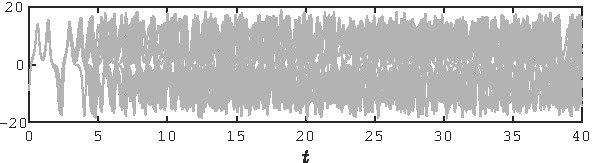
\includegraphics[]{LorenzTest1} \\
			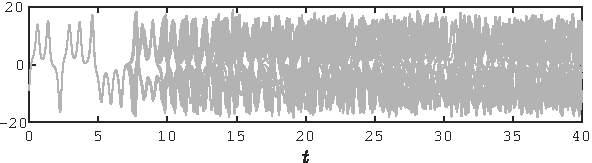
\includegraphics[]{LorenzTest2} \\
 			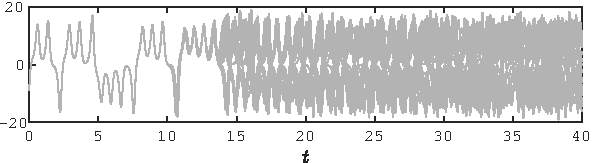
\includegraphics[]{LorenzTest3}
		\end{tabular}
	\end{center}
	\caption{Uncertainty quantification on the first component of the Lorenz system performed with the RTS-RK method (first figure), and by random perturbation perturbation of the initial condition (second and third figures).}
	\label{fig:LorenzTest}
\end{figure}

\subsection{Robustness} In this numerical experiment we verify the robustness of RTS-RK when applied to chemical reactions. Let us consider the Peroxide-Oxide chemical reaction, which is macroscopically defined by the following balance equation
\begin{equation}
	\mathrm{O}_2 + 2\mathrm{NADH} + 2\mathrm{H}^+ \to 2\mathrm{H}_2\mathrm{O} + 2\mathrm{NAD}^+.
\end{equation}
This reaction has to be catalyzed by an enzyme to take place, which reacts with the reagents to create intermediate products of the reaction. A successful model \cite{Ols83} to describe the time-evolution of the chemical system is the following
\begin{equation}
\begin{aligned}
	\mathrm{B} + \mathrm{X} &\rightarrowtext{k_1} 2 \mathrm{X}, 
	&&2\mathrm{X} \rightarrowtext{k_2} 2\mathrm{Y}, 
	&&\mathrm{A} + \mathrm{B} + \mathrm{Y} \rightarrowtext{k_3} 3 \mathrm{X}, \\
	\mathrm{X} &\rightarrowtext{k_4} \mathrm{P}, 
	&&\mathrm{Y} \rightarrowtext{k_5} \mathrm{Q}, 
	&&\mathrm{X_0} \rightarrowtext{k_6} \mathrm{X}, \\
	\mathrm{A_0} &\leftrightarrowtext{k_7} \mathrm{A}, 
	&&\mathrm{B_0} \rightarrowtext{k_8} \mathrm{B}.
\end{aligned}
\end{equation}
Here, A and B are respectively $[\mathrm{O}_2]$ and $[\mathrm{NADH}]$, P, Q are the products and X, Y are intermediates results of the reaction process. It is therefore possible to model the time evolution of the reaction with the following system of nonlinear ODEs 
\begin{equation}\label{eq:PeroxOx}
\begin{aligned}
	\mathrm{A}' &= k_7  (\mathrm{A}_0 - \mathrm{A}) - k_3  \mathrm{A}\mathrm{B}\mathrm{Y}, &&\mathrm{A}(0) = 6, \\
	\mathrm{B}' &= k_8\mathrm{B}_0 - k_1  \mathrm{B}\mathrm{X} - k_3  \mathrm{A}\mathrm{B}\mathrm{Y}, &&\mathrm{B}(0) = 58, \\
	\mathrm{X}' &= k_1  \mathrm{B}\mathrm{X} - 2  k_2  \mathrm{X}^2 + 3  k_3 \mathrm{A}\mathrm{B}\mathrm{Y} - k_4  \mathrm{X} + k_6\mathrm{X}_0,&& \mathrm{X}(0) = 0, \\
	\mathrm{Y}' &= 2  k_2  \mathrm{X}^2 - k_5  \mathrm{Y} - k_3  \mathrm{A}\mathrm{B}\mathrm{Y}, && Y(0) = 0,
\end{aligned}
\end{equation}
where $\mathrm{A}_0 = 8$, $\mathrm{B}_0 = 1$, $\mathrm{X}_0 = 1$ and the real parameters $k_i$, $i = 1, \ldots, 8$ representing the reaction rates take values
\begin{equation}
\begin{aligned}
k_1 &= 0.35, &&k_2 = 250, &&k_3 = 0.035, &&k_4 = 20,\\
k_5 &= 5.35, &&k_6 = 10^{-5}, &&k_7 = 0.1, &&k_8 = 0.825.
\end{aligned}
\end{equation}            
It has been shown \cite{Ols83} that for these values of the parameters the system exhibits a chaotic behavior. In particular, at long time the trajectories are captured in a strange attractor, and the system shows a strong sensitivity to perturbations on the initial condition. 

Since the components of the solution represent the concentration of chemicals, we require the numerical solution to be positive. Apart from physical considerations, numerically we observe that if one of the components takes negative values, the solution shows strong instabilities. Let us consider the maximum time step $h_{\max}$ for which the deterministic numerical solution stays positive and thus is stable. The probability that the RTS-RK method presents instabilities before time $T = hN$ depends on the distribution of the variables $H_k$. In some situations this probability can be computed explicitly. For example, if they are drawn from a uniform distribution as in Example \ref{ex:uniformH}, we can just set $h + h^p < h_{\max}$ thus having a null probability of being unstable. In contrast, for the additive noise method we can have disruptive effects even with small time steps if the solution has a small magnitude. To illustrate this issue, let us consider a one-dimensional problem solved by the additive noise method \eqref{eq:ProbMethAddNoise} with $\xi_k(h)$ i.i.d. random variables $\mathcal{N}(0, h^{2p + 1})$. With this choice of random variables, even in case the underlying deterministic method with time step $h$ would give a positive value, the probability of the probabilistic numerical solution to turn negative is always greater than zero. In particular, if the magnitude of the numerical solution $Y_k$ is close to zero then the probability of the event $(Y_{k+1} < 0)$ is significant. Hence, integrating over long time an equation whose components should stay positive with a small magnitude employing the additive noise method likely produces instabilities regardless of the chosen time step.

Let us apply the additive noise method \eqref{eq:ProbMethAddNoise} and the random time-stepping scheme \eqref{eq:ProbMethVarH} to equation \eqref{eq:PeroxOx}. We choose $h = 0.05$ as the mean time steps for \eqref{eq:ProbMethVarH} and as the time step for \eqref{eq:ProbMethAddNoise}, while we employ the Runge-Kutta-Chebyshev method (RKC) \cite{HoS80} as deterministic integrator. The RKC method is a stabilized numerical integrator of first order, which allows to obtain stable solutions with an explicit scheme. Higher order explicit stabilized methods such as ROCK2 or ROCK4 \cite{AbM01, Abd02} could also be used as deterministic solvers for the RTS-RK method. It can be seen in Figure \ref{fig:OxPeroxTraj} that the RTS-RK method conserves the positivity of the numerical solution while capturing the chaotic nature of the chemical reaction, while the additive noise scheme produces negative values, thus showing strong instabilities in the long-time behavior.
\begin{figure}
	\begin{center} 
		\begin{tabular}{c}
			\includegraphics[]{OxPerox}\\
			\hspace{0.25cm}\includegraphics[]{OxPeroxAdd}
		\end{tabular}
	\end{center}
	\caption{Thirty trajectories of the numerical value of the concentration of the X species for the random time-stepping and additive noise methods (above and below respectively).}
	\label{fig:OxPeroxTraj}
\end{figure}

\subsection{Conservation of quadratic first integrals} 

\begin{figure}[t]
	\begin{center}
		\begin{tabular}{c@{\hspace{0.3cm}}c}
			\includegraphics[]{KeplerOne} & \includegraphics[]{KeplerTwo} \\
			\includegraphics[]{KeplerOneAdd} & \includegraphics[]{KeplerTwoAdd} \\
		\end{tabular}
	\end{center}
	\hspace{0.84cm}\includegraphics[]{KeplerMom}
	\caption{Trajectories of \eqref{eq:KeplerPert} given by the RTS-RK method \eqref{eq:ProbMethVarH} for $0 \leq t \leq 200$ and $3800 \leq t \leq 4000$ (first row, left and right), and by the additive noise method \eqref{eq:ProbMethAddNoise} for $0 \leq t \leq 200$ and $200 \leq t \leq 400$ (second row, left and right). Error on the angular momentum for $0 \leq t \leq 4000$ given by the two methods.}
	\label{fig:Kepler}
\end{figure}

A simple model for the two-body problem in celestial mechanics is the Kepler system with a perturbation, , which reads
\begin{equation}\label{eq:KeplerPert}
\begin{aligned}
	q_1' &= p_1, && p_1' = -\frac{q_1}{\norm{q}^3} - \frac{\delta q_1}{\norm{q}^5}, \\
	q_2' &= p_2, && p_2' = -\frac{q_2}{\norm{q}^3} - \frac{\delta q_2}{\norm{q}^5},
\end{aligned}
\end{equation}
where $p_1$, $p_2$ are the two components of the velocity and $q_1$, $q_2$ are the two components of the position. We assume the perturbation parameter $\delta$ to be equal to 0.015 and the initial condition to be
\begin{equation}
	q_1(0) = 1 − e,\quad q_2(0) = 0, \quad p_1(0) = 0, \quad p_2(0) = \sqrt{(1 + e)/(1 − e)},
\end{equation}
where $e = 0.6$ is the eccentricity. It is well-known that this equation has the Hamiltonian and the angular momentum as quadratic first integrals. In particular, we focus here on the angular momentum, which reads
\begin{equation}
	I(p, q) = q_1p_2 - q_2p_1.
\end{equation}
We consider the simplest Gauss collocation method, namely the implicit midpoint rule, as the deterministic Runge-Kutta method. It is known that Gauss collocation methods conserve quadratic first integrals. According to Theorem \ref{thm:PolyInvariants}, we expect therefore that the random time-stepping method \eqref{eq:ProbMethVarH} implemented with $\Psi_h$ given by the implicit midpoint rule conserves also quadratic first integrals. We therefore integrate \eqref{eq:KeplerPert} with mean time step $h = 0.01$ from time $t = 0$ to time $t = 4000$ which corresponds to approximately $636$ revolutions of the system (long-time behavior). Moreover, we consider the additive noise method \eqref{eq:ProbMethAddNoise} with $h = 0.01$, expecting that the first integral will not be conserved. We observe in Figure \ref{fig:Kepler} that the method \eqref{eq:ProbMethVarH} conserves the angular momentum, while for the method \eqref{eq:ProbMethAddNoise} the approximate conservation of the quadratic first integral shown in \eqref{eq:BiasQuadraticAddNoise} is lost when integrating \eqref{eq:KeplerPert} over long time.

\subsection{Chaotic Hamiltonian systems}\label{sec:Lorenz}

\begin{figure}[t!]
	\begin{center}
		\begin{tabular}{cc}
			\includegraphics[]{HHStep} & \includegraphics[]{HHAdd} \\
		\end{tabular}
		\begin{tabular}{c}
			\includegraphics[]{HHStepChaos} \\
			\includegraphics[]{HHStepHam}
		\end{tabular}
	\end{center}
	\caption{A trajectory of \eqref{eq:HenHei} given by the RTS-RK method \eqref{eq:ProbMethVarH} for $0 \leq t \leq 350$ (first row, left), and by the additive noise method \eqref{eq:ProbMethAddNoise} (first row, right). Value of $q_1$ for the whole set of realizations of \eqref{eq:ProbMethVarH} for $0 \leq t \leq 600$. Error on the Hamiltonian $H(p_0, q_0) = 0.13$ for $0 \leq t \leq 600$.}
	\label{fig:HH}
\end{figure}

Probabilistic methods for differential equations are of particular interest when applied to chaotic systems. Hamiltonian systems can present chaotic features in the long-time behavior, while conserving geometric properties. It is therefore relevant to study whether both the geometric features and the chaotic nature are captured by the probabilistic integrator. An example of this class of system is given by the Hénon-Heiles problem \cite{HeH64}, whose Hamiltonian (total energy) is given by
\begin{equation}\label{eq:HenHeiHam}
	H(p, q) = \frac{1}{2}\norm{p}^2 + \frac{1}{2}\norm{q}^2 + q_1^2q_2 - \frac{1}{3}q_2^3,
\end{equation}
where $p$ and $q$ are vectors of $\R^2$ representing velocity and position respectively. The corresponding system of ODEs can then be written as
\begin{equation}\label{eq:HenHei}
\begin{aligned}
	p' &= -\nabla_q H(p, q), &&p(0) = p_0 \in \R^2,\\
	q' &= \nabla_p H(p, q), &&q(0) = q_0 \in \R^2.
\end{aligned}
\end{equation}
It is well-known that this systems presents typical deterministic chaos for values $H > 1/8$. We pick as deterministic integrator the $s$-stage trapezoidal rule \cite{IaT09}. It has been proved that this numerical scheme conserves polynomial Hamiltonians of degree less than $s$ for $s$ even, or $s + 1$ for $s$ odd. Thanks to Theorem \ref{thm:PolyInvariants}, if we choose as the $s$-stage trapezoidal rule, with $s \geq 4$, as the deterministic component $\Psi_h$ of \eqref{eq:ProbMethVarH}, {we expect the Hamiltonian \eqref{eq:HenHeiHam} to be conserved exactly for all the numerical trajectories. However, we do not expect the additive noise method \eqref{eq:ProbMethAddNoise} to conserve the Hamiltonian in this case.

For this numerical experiment, we assume the initial condition to be
\begin{equation}
	q_1(0) = 0.5,\quad q_2(0) = 0, \quad p_1(0) = 0, \quad p_2(0) = 0.1,
\end{equation}
so that the Hamiltonian is $H = 0.13 > 1/8$ and \eqref{eq:HenHei} is in the chaotic regime. We then integrate the equation for time $t \in [0, 600]$ with the two probabilistic versions of the $5$-stage trapezoidal rule choosing as mean time step $h = 0.01$ for \eqref{eq:ProbMethVarH} and fixing $h = 0.01$ for \eqref{eq:ProbMethAddNoise}. We compute $M = 10$ trajectories for both the numerical methods. The results given in Figure \ref{fig:HH} show that each trajectory given by the random time-stepping technique conserves the Hamiltonian function, nonetheless capturing the chaotic behavior of the system at long time (Figure \ref{fig:HH}, second row). In fact, after a short time where all trajectories approximately coincide, the attractor in the phase space is explored fully by the set of trajectories. In contrast, the additive noise method does not conserve the Hamiltonian, with all trajectories presenting an energy deviation from the initial value. Due to this deviation, all trajectories present an unstable behavior after a short time, while the random time-stepping technique is stable for the same value of $h$.

\subsection{Hamiltonian systems} 

\begin{figure}[t!]
	\begin{center}
		\begin{tabular}{c}
			\includegraphics[]{Ham1} \\
			\includegraphics[]{Ham2}
		\end{tabular}
	\end{center}
	\caption{Energy of the harmonic oscillator for the RTS-RK (first picture) and the deterministic (second picture) Störmer-Verlet schemes. In the first picture, light grey lines represent the energy along realisations of the probabilistic solution, while the black line represents the mean value of $E(t)$.}
	\label{fig:Ham}
\end{figure}

A class of dynamical systems of particular interest for their geometric properties are the Hamiltonian systems. Given a function $E(p, q)$, called the Hamiltonian, with $p$ and $q$ in $\R^d$, they can be written as
\begin{equation}\label{eq:ODEHam}
	y' = J^{-1}\nabla E(y), \quad y(0) = y_0,
\end{equation}
where $y = (p, q)^\top$ and the matrix $J\in\R^{2d \times 2d}$ is defined as
\begin{equation}
	J = \begin{pmatrix} \mathbf{0} & I \\ -I & \mathbf{0} \end{pmatrix},
\end{equation}
and where $I$ and $\mathbf{0}$ are respectively the identity and the zero matrices in $\R^{d\times d}$. It is well-known that the flow $\phi_t\colon\R^{2d}\to\R^{2d}$ of any system of the form \eqref{eq:ODEHam} is symplectic, i.e., 
\begin{equation}\label{eq:SymplecticSystem}
	\pdv{\phi_t(y)}{y}^\top J \pdv{\phi_t(y)}{y} = J, \quad \forall y \in \R^d,
\end{equation}
where we denote by $y\in \R^{2d}$ the vector $(p, q)^\top$. Condition \eqref{eq:SymplecticSystem} is equivalent in a geometric sense to saying that the flow $\phi_t$ of the system conserves areas in the phase space. In a natural manner, the flow $\Psi_h$ of a one-step numerical method for \eqref{eq:ODEHam} is called symplectic it satisfies
\begin{equation}\label{eq:SymplecticMethod}
	\pdv{\Psi_h(y)}{y}^\top J \pdv{\Psi_h(y)}{y} = J.
\end{equation}
It has been pointed out \cite{SkG92, HLW06} that applying an adaptive step size technique to a symplectic method can destroy its simplecticity. Therefore, Skeel and Gear \cite{SkG92} write any adaptive technique in function of a map $\tau(y, h)$ such that the $k$-th time step $h_k$ is selected as $h_k = \tau(y_k, h)$, where $h$ is a base value for the time step. Hence, in order to have again a symplectic method, the new condition to be satisfied is
\begin{equation}\label{eq:SymplecticCondition}
	V^\top J V = J, \quad V = \pdv{\Psi_{\tau(y, h)}(y)}{y} + \pdv{\Psi_{\tau(y, h)}(y)}{t}\pdv{\tau(y, h)}{y}^\top.
\end{equation}
Let us now consider the RTS-RK method based on a symplectic deterministic integrator. We have the following lemma. 
\begin{lemma}\label{lem:SympRTSRK} If the flow $\Psi_h$ of the deterministic integrator is symplectic, then the flow of the random time-stepping probabilistic method \eqref{eq:ProbMethVarH} is symplectic.
\end{lemma}
\begin{proof} For the RTS-RK scheme, the $k$-th time step $H_k$ is selected via a random mapping $\tau(y, h) = \tau(h) = h\Theta_k$, where $\Theta_k$ are opportunely scaled random variables such that $H_k$ satisfies Assumption \ref{as:hStrong}. Hence, $\tau$ is independent of $y$ and with the notation introduced above 
\begin{equation}
	V = \pdv{\Psi_{\tau(h)}(y)}{y}.
\end{equation}
Therefore, by the symplecticity of $\Psi_t$ the condition $V^\top J V = J$ is satisfied and the flow map of the RTS-RK method is symplectic.
\end{proof}

While Lemma \ref{lem:SympRTSRK} shows that the flow map of the RTS-RK method is symplectic one has to be careful on the conclusion drawn from this property. Indeed, for deterministic integrators it is possible to show via backwards analysis near conservation of the total energy of a Hamiltonian system \cite{SaC94,HaL97,LeR01}. For the RTS-RK the classical backward error analysis cannot be applied and conservation of the total energy for a simple trajectory does not hold in general. It seems however that the total energy might be preserved in the mean sense as shown in the following example.

Consider by the harmonic oscillator, which is given by the Hamiltonian $E(p, q) = (p^2 + q^2) / 2$. We integrate the harmonic oscillator to final time $T = 4000$ employing the symplectic Störmer-Verlet scheme, both with fixed time step $h = 0.4$ and with the RTS-RK method based on the same deterministic integrator and with mean time step $h$. We choose an initial condition such that $E(p_0, q_0) = 1$. Results, displayed in Figure \ref{fig:Ham}, show that the value of $E$ deviates from its initial value along the realisations of the RTS-RK scheme, while the same method with fixed time steps oscillates around the true value of $E$. As mentioned above, the RTS-RK method seems to conserve the Hamiltonian in the mean sense, but the analysis of this phenomenon will be reported elsewhere.

\subsection{Bayesian inferential problems}\label{sec:BayesianInferenceEx}

\begin{figure}[t!]
	\begin{center}
		\begin{tabular}{c@{\hspace{0.3cm}}c}
			\includegraphics[]{PostDet} & \includegraphics[]{PostProb} \\ 
		\end{tabular}
	\end{center}
	\caption{Posterior distribution for $\exp(\theta_3)$ obtained with the standard random walk Metropolis and the explicit Euler method (left picture) and the pseudo-marginal Metropolis-Hastings and RTS-RK explicit Euler method (right picture). In the plot, $h_i = 0.1\cdot 2^{-i}$. The dashed vertical line indicates the true value of the parameter $\exp(\theta^*_3)$.}
	\label{fig:MCMC}
\end{figure}

For the last numerical experiment we revisit the FitzHug-Nagumo equation,
\begin{equation}\label{eq:FitzNag2}
\begin{aligned}
y_{\theta, 1}' &= c\big(y_{\theta, 1} - \frac{y_{\theta, 1}^3}{3} + y_{\theta, 2}\big), && y_{\theta, 1}(0) = -1, \\
y_{\theta, 2}' &= -\frac{1}{c}(y_{\theta, 1} - a + b y_{\theta, 2}), && y_{\theta, 2}(0) = 1,
\end{aligned}
\end{equation}
where in the spirit of Bayesian inverse problems we consider $a, b, c \in \R$ to be unknown parameters. We recall that their true value is given by $a = 0.2$, $b = 0.2$ and $c = 3$, see equation \eqref{eq:FitzNag}. The test is then to infer the value of the parameter $\theta = (\theta_1, \theta_2, \theta_3)^\top = (\log a, \log b, \log c)^\top \in \R^3$ from observations of the solution of \eqref{eq:FitzNag2}. The exponential transformation operated on each component of the parameter is taken to ensure positiveness of $(a, b, c)^\top$ for any value of $\theta$.  We consider the forward problem operator $\mathcal{G} \colon \R^n \to \R^m$ introduced in Section \ref{sec:BayesianInference} to be defined by
\begin{equation}
	\mathcal{G}(\theta) = (y_\theta(0.1)^\top,\, y_\theta(0.2)^\top, \ldots,\, y_\theta(1)^\top)^\top,
\end{equation} 
thus $n = 3$ and $m = 20$. Synthetic observations are then generated fixing $\theta$ to its true value $\theta^* = (\log(0.2), \log(0.2), \log(3))^\top$ and integrating the equation with a Runge-Kutta solver with a small time step and biased by Gaussian observational noise, i.e.,
\begin{equation}
	\mathcal{Y} = \mathcal{G}(\theta) + \eta, \quad \eta \sim \mathcal{N}\big(0, (0.05)^2 I_{20}\big),
\end{equation}
where $I_{r}$ is the $r$-dimensional identity matrix. We fix the prior distribution on $\theta$ to be a standard Gaussian $\mathcal{N}(0, I_3)$. Let us remark that since the amount of noise in the observational model is small, this choice of prior does not yield information on the true value of the parameter. We then sample from the posterior distributions $\pi^h(\theta \mid \mathcal Y)$ and $\pi^h_{\mathrm{pr}}(\theta \mid \mathcal Y)$ employing the sampling methods described in Section \ref{sec:Sampling}, namely
\begin{enumerate}
	 \item the standard RWM with the forward map approximated by the explicit Euler method,
	 \item the PMMH with the forward map approximated via RTS-RK implemented with the explicit Euler method.
\end{enumerate}
In both cases, we perform the MCMC algorithm four times, varying the step size $h$ (or mean step size for RTS-RK), precisely choosing $h_i = 0.1\cdot2^{-i}$, $i = 0, 1, 2, 3, 4$. We recall that for the PMMH algorithm the stationary distribution of the generated Markov chain is independent of the number of samples chosen to approximate the posterior at each iteration with Monte Carlo. In order to get an initial value for the Markov chain in the PMMH case, we perform a short trial run of the MCWM method to move towards sets with significant values of the posterior density. In Figure \ref{fig:MCMC} we show the marginal posterior for the parameter $\exp(\theta_3)$. We observe that while for the standard deterministic approximation of $\mathcal{G}$ the coarser values of $h$ provide an overconfident posterior centred in a biased value, the same computation performed with RTS-RK and PMMH accounts better for the statistical uncertainty introduced by the discretisation error.

\def\cprime{$'$}
\begin{thebibliography}{10}
	
	\bibitem{Abd02}
	{\sc A.~Abdulle}, {\em Fourth order {C}hebyshev methods with recurrence
		relation}, SIAM J. Sci. Comput., 23 (2002), pp.~2041--2054.
	
	\bibitem{AbM01}
	{\sc A.~Abdulle and A.~A. Medovikov}, {\em Second order {C}hebyshev methods
		based on orthogonal polynomials}, Numer. Math., 90 (2001), pp.~1--18.
	
	\bibitem{AnR09}
	{\sc C.~Andrieu and G.~O. Roberts}, {\em The pseudo-marginal approach for
		efficient {M}onte {C}arlo computations}, Ann. Statist., 37 (2009),
	pp.~697--725.
	
	\bibitem{CCC16}
	{\sc O.~A. Chkrebtii, D.~A. Campbell, B.~Calderhead, M.~A. Girolami, et~al.},
	{\em Bayesian solution uncertainty quantification for differential
		equations}, Bayesian Anal., 11 (2016), pp.~1239--1267.
	
	\bibitem{COS17}
	{\sc J.~Cockayne, C.~Oates, T.~Sullivan, and M.~Girolami}, {\em Probabilistic
		numerical methods for {PDE}-constrained {B}ayesian inverse problems}, AIP
	Conference Proceedings, 1853 (2017), p.~060001.
	
	\bibitem{CGS16}
	{\sc P.~R. Conrad, M.~Girolami, S.~S{\"a}rkk{\"a}, A.~Stuart, and
		K.~Zygalakis}, {\em Statistical analysis of differential equations:
		introducing probability measures on numerical solutions}, Stat. Comput.,
	(2016).
	
	\bibitem{HaL97}
	{\sc E.~Hairer and C.~Lubich}, {\em The life-span of backward error analysis
		for numerical integrators}, Numer.\ Math., 76 (1997), pp.~441--462.
	\newblock Erratum: http://www.unige.ch/math/folks/hairer/.
	
	\bibitem{HLW06}
	{\sc E.~Hairer, C.~Lubich, and G.~Wanner}, {\em Geometric Numerical
		Integration. Structure-Preserving Algorithms for Ordinary Differential
		Equations}, Springer Series in Computational Mathematics 31, Springer-Verlag,
	Berlin, second~ed., 2006.
	
	\bibitem{HNW93}
	{\sc E.~Hairer, S.~P. N{\o{}}rsett, and G.~Wanner}, {\em Solving Ordinary
		Differential Equations I. Nonstiff Problems}, vol.~8, Springer Verlag Series
	in Comput. Math., Berlin, 1993.
	
	\bibitem{HaW96}
	{\sc E.~Hairer and G.~Wanner}, {\em Solving ordinary differential equations II.
		Stiff and differential-algebraic problems}, Springer-Verlag, Berlin and
	Heidelberg, 1996.
	
	\bibitem{HeH64}
	{\sc M.~H\'enon and C.~Heiles}, {\em The applicability of the third integral of
		motion: {S}ome numerical experiments}, Astronom. J., 69 (1964), pp.~73--79.
	
	\bibitem{IaT09}
	{\sc F.~Iavernaro and D.~Trigiante}, {\em High-order symmetric schemes for the
		energy conservation of polynomial {H}amiltonian problems}, JNAIAM J. Numer.
	Anal. Ind. Appl. Math., 4 (2009), pp.~87--101.
	
	\bibitem{KaS05}
	{\sc J.~Kaipio and E.~Somersalo}, {\em Statistical and Computational Inverse
		Problems}, Applied Mathematical Sciences, 160, Springer, 2005.
	
	\bibitem{KeH16}
	{\sc H.~Kersting and P.~Hennig}, {\em Active uncertainty calibration in
		{B}ayesian {ODE} solvers}, in Proceedings of the 32nd Conference on
	Uncertainty in Artificial Intelligence (UAI 2016), {AUAI} Press, 2016,
	pp.~309--318.
	
	\bibitem{LeR01}
	{\sc B.~Leimkuhler and S.~Reich}, {\em A reversible averaging integrator for
		multiple time-scale dynamics}, J. Comput. Phys., 171 (2001), pp.~95--114.
	
	\bibitem{Lor63}
	{\sc E.~N. Lorenz}, {\em Deterministic nonperiodic flow}, J. Atmos. Sci., 20
	(1963), pp.~130--141.
	
	\bibitem{MLR16}
	{\sc F.~J. Medina-Aguayo, A.~Lee, and G.~O. Roberts}, {\em Stability of noisy
		{M}etropolis--{H}astings}, Stat. Comput., 26 (2016), pp.~1187--1211.
	
	\bibitem{Ols83}
	{\sc L.~F. Olsen}, {\em An enzyme reaction with a strange attractor}, Phys.
	Lett. A, 94 (1983), pp.~454 -- 457.
	
	\bibitem{SaC94}
	{\sc J.~M. Sanz-Serna and M.~P. Calvo}, {\em Numerical {H}amiltonian
		{P}roblems}, Chapman \& Hall, London, 1994.
	
	\bibitem{SkG92}
	{\sc R.~D. Skeel and C.~W. Gear}, {\em Does variable step size ruin a
		symplectic integrator?}, Physica, 60 (1992), pp.~311--313.
	
	\bibitem{Stu10}
	{\sc A.~M. Stuart}, {\em Inverse problems: A {B}ayesian perspective}, Acta
	Numer., 19 (2010), pp.~451--559.
	
	\bibitem{HoS80}
	{\sc P.~van~der Houwen and B.~P. Sommeijer}, {\em On the internal stage
		{R}unge-{K}utta methods for large m-values}, Z. Angew. Math. Mech., 60
	(1980), pp.~479--485.
	
\end{thebibliography}

\end{document}
